\documentclass[12pt,a4paper]{article}
\usepackage[T1]{fontenc}
\usepackage[utf8]{inputenc}
\usepackage{lmodern,microtype}
\usepackage[a4paper,left=25mm,right=25mm,top=23mm,textheight=672pt]{geometry}
\usepackage{amsmath,amssymb,amsthm,bm,mathtools}
\usepackage{graphicx,booktabs,array,longtable}
\usepackage[round,authoryear]{natbib}
\usepackage{setspace}
\usepackage{hyperref,xurl}
\hypersetup{hidelinks,pdfauthor={Jian Hou, Tan Meng, Maozai Tian}}
\usepackage[font=normalsize,labelfont=bf]{caption}
\newtheorem{theorem}{Theorem}
\newtheorem{proposition}{Proposition}
\newtheorem{lemma}{Lemma}
\newtheorem{corollary}{Corollary}
\theoremstyle{definition}\newtheorem{assumption}{Assumption}
\newtheorem{remark}{Remark}
\DeclareMathOperator{\Var}{Var}\DeclareMathOperator{\Cov}{Cov}
\DeclareMathOperator{\tr}{tr}\DeclareMathOperator{\argmin}{arg\,min}\DeclareMathOperator{\argmax}{arg\,max}
\newcommand{\E}{\mathbb E}\newcommand{\PP}{\mathbb P}\newcommand{\R}{\mathbb R}\newcommand{\ind}{\mathbf 1}
\newcommand{\op}{\mathrm{op}}\newcommand{\sg}{\mathrm{G}}\newcommand{\se}{\mathrm{E}}
\newcommand{\sT}{\mathrm{T}}\newcommand{\Yset}{\mathcal Y}\newcommand{\Lset}{\Lambda}
\newcommand{\wh}{\widehat}\newcommand{\wt}{\widetilde}\newcommand{\norm}[1]{\left\lVert#1\right\rVert}
\newcommand{\inner}[2]{\langle #1,#2\rangle}\newcommand{\Pp}{\mathbb P_n}
\newcommand{\mc}{\mathrm{mc}}\newcommand{\parens}[1]{\left(#1\right)}
\setlength{\parindent}{1.25em}\setlength{\parskip}{0pt}
\setlength{\emergencystretch}{2em}
\graphicspath{{../figures/}}
\doublespacing

% Float placement preserves the body font and line spacing.
\renewcommand{\topfraction}{0.9}
\renewcommand{\bottomfraction}{0.8}
\renewcommand{\textfraction}{0.08}
\renewcommand{\floatpagefraction}{0.65}
\setcounter{topnumber}{3}
\setcounter{bottomnumber}{2}

\makeatletter
\renewcommand*\l@section{\@dottedtocline{1}{0em}{2.8em}}
\renewcommand*\l@subsection{\@dottedtocline{2}{2.8em}{3.3em}}
\makeatother
\newcommand{\SimCovMin}{0.944}
\newcommand{\SimCovMax}{0.968}
\newcommand{\SimAlignedWidthMin}{0.731}
\newcommand{\SimAlignedWidthMax}{0.831}
\newcommand{\SimReversalWeight}{0.000}
\newcommand{\SimHarmMax}{0.000}
\newcommand{\EpaWidthMin}{0.746}
\newcommand{\EpaWidthMax}{1.000}
\newcommand{\EpaJointMin}{0.935}
\newcommand{\EpaJointMax}{0.970}
\newcommand{\NumAgreement}{1.000}
\newcommand{\NumCriticalError}{0.000}
\newcommand{\NumGainError}{0.000}
\newcommand{\NumCovError}{0.000}

\renewcommand{\thesection}{S\arabic{section}}
\renewcommand{\theequation}{S\arabic{equation}}
\renewcommand{\thetheorem}{S\arabic{theorem}}
\renewcommand{\theproposition}{S\arabic{proposition}}
\renewcommand{\thelemma}{S\arabic{lemma}}
\renewcommand{\thecorollary}{S\arabic{corollary}}
\renewcommand{\thetable}{S\arabic{table}}
\renewcommand{\thefigure}{S\arabic{figure}}
\title{Supplement to ``Surrogate-assisted local conditional distribution inference with certified simultaneous gains''}
\author{Jian Hou, Tan Meng, and Maozai Tian}\date{}
\begin{document}\maketitle
\noindent This Supplement supplies proofs and implementation details for the revised method. References to numbered theorems without an S prefix refer to the main manuscript. The independent-role population experiment and the fixed-frame Bernoulli audit have different covariance estimators; both are derived explicitly.
\tableofcontents
\section{Geometry of paired critical values}
\subsection{Notation and exact local identities}
All expectations in Sections S1--S5 are conditional on the independent training sample. Dependence on the triangular row is suppressed. The threshold grid is $y_1<\cdots<y_J$. Set $Z_j=\ind(Y\leq y_j)$, $D=m-q$, $a_\lambda=q+\lambda D$, and
\[
 U_\lambda=a_\lambda+R\pi^{-1}(Z-a_\lambda),\qquad
 B=(1-R/\pi)D.
\]
With $R\perp Y\mid W$ and $\E(R\mid W)=\pi$, conditioning on $(W,Y)$ gives
$\E(U_\lambda\mid W,Y)=Z$ and $\E(B\mid W,Y)=0$.
Consequently $\E K_h(U_\lambda-F_h)=0$. For $n$ evaluation observations,
\begin{align}
 \sqrt{npv_h}(\wh F_\lambda-F_h)
 &=\frac{\sqrt{npv_h}\,n^{-1}\sum_i K_i(U_{\lambda,i}-F_h)}{\overline K}\notag\\
 &=\frac{n^{-1/2}\sum_i\sqrt{p/v_h}K_i(U_{\lambda,i}-F_h)}{\overline K/v_h}.
\end{align}
Thus denominator estimation need not be approximated for the coverage event: multiplying the estimated half-width by the same positive denominator cancels it exactly.

\subsection{Proof of the separation proposition}
The four $(S,Y)$ states $(0,1),(0,2),(1,0),(1,2)$ have probabilities $0.4,0.4,0.1,0.1$. The two candidate vectors are $(0,0.42)$ and $(0.5,0.82)$; each extends to a genuine cumulative distribution by taking value zero below zero and one at and above two. Enumerating these states and the independent verification indicator gives
\begin{equation}\label{eq:s-separation}
 \Sigma_\lambda=
 \begin{pmatrix}
 .09-.072\lambda+.036\lambda^2&.05-.0288\lambda+.0288\lambda^2\\
 .05-.0288\lambda+.0288\lambda^2&.25+.02304\lambda^2
 \end{pmatrix}.
\end{equation}
Its trace is $.34-.072\lambda+.05904\lambda^2$, with minimiser $25/41$. At zero borrowing, the union bound gives
\[
 \Pr(\|G_0\|_\infty>.99)
 \leq2\overline\Phi(.99/.3)+2\overline\Phi(.99/.5)
 =.04867037697<.05.
\]
At $25/41$, the second variance is $.25856632957$, so
\[
 \Pr(\|G_{25/41}\|_\infty\leq.99)
 \leq2\Phi\{.99/\sqrt{.25856632957}\}-1
 =.94845626635<.95.
\]
Therefore $c_\Omega(0)<.99<c_\Omega(25/41)$. Deterministic bivariate integration gives the values in the main text; numerical minimisation of the band criterion gives $\lambda=0.114860$ and $c=0.982639$. These latter values are not needed for the strict separation. An independent continuous $X$ and a common kernel embed the example into a local conditional distribution, multiplying every covariance by the same positive constant.

\subsection{Gaussian-quantile differentiability}
Let $q_\alpha(\Sigma)$ denote the $(1-\alpha)$ quantile of $\|N(0,\Sigma)\|_\infty$. Define
\[
 H(t,\Sigma)=\int_{[-t,t]^J}\phi_\Sigma(z)\,dz,\qquad t>0.
\]
On any compact subset of the positive definite cone, Gaussian density derivatives of every finite order are dominated by a polynomial times an integrable Gaussian. Differentiation under the integral is therefore valid. Substitution $z=tu$, $u\in[-1,1]^J$, gives joint smoothness in $t$ and $\Sigma$. The derivative in $t$ is a sum of strictly positive face integrals, so $H_t(t,\Sigma)>0$. Also $H(0,\Sigma)=0$ and $H(t,\Sigma)\to1$. The implicit function theorem applied to $H(q,\Sigma)=1-\alpha$ shows that $q_\alpha$ is infinitely continuously differentiable.

For a symmetric direction $E$, its first derivative is
\begin{equation}\label{eq:gradientq}
 Dq_\alpha(\Sigma)[E]=-
 \frac{\frac12\int_{[-q,q]^J}\phi_\Sigma(z)
 \{z^\top\Sigma^{-1}E\Sigma^{-1}z-\tr(\Sigma^{-1}E)\}\,dz}
 {H_t(q,\Sigma)}.
\end{equation}
The quantile remains in a compact positive interval when the eigenvalues of $\Sigma$ range over $[\kappa,2B]$. Continuity and compactness give finite bounds $M_r$ for its derivatives of orders $r=1,2,3$. They depend on $J,\alpha,\kappa,B$.

\subsection{Proofs of Theorems 1 and 2}
On $\Omega\in\mathcal C_G$, the true gain dominates its lower bound at every weight. Since zero is a candidate, $L_G(\lambda_G)\geq L_G(0)=0$. This proves the certificate. Moreover,
\[
 g_\Omega(\lambda_G)\geq L_G(\lambda_G)
 \geq L_G(\lambda^\star)
 \geq g_\Omega(\lambda^\star)-\sup_{Q\in\mathcal C_G}|g_Q(\lambda^\star)-g_\Omega(\lambda^\star)|.
\]
Optimality of $\lambda^\star$ supplies the lower side of the regret inequality. A finite grid guarantees existence and measurability after deterministic tie-breaking.

For Theorem 2, write $f_\lambda(Q)=q_\alpha(H_\lambda QH_\lambda^\top)$ and $\Sigma_\lambda=H_\lambda QH_\lambda^\top$. Since $\|H_\lambda\|_\op^2\leq2$,
\[
 \|H_\lambda EH_\lambda^\top-H_0EH_0^\top\|_\op\leq3\lambda\|E\|_\op,
 \qquad \|\Sigma_\lambda-\Sigma_0\|_\op\leq3B\lambda.
\]
The chain rule and the bounds $M_1,M_2$ yield
\[
 |D(f_0-f_\lambda)(Q)[E]|
 \leq(3M_1+6BM_2)\lambda\|E\|_\op.
\]
The class $\mathcal K_{\kappa,B}$ is convex, so integrating along the segment between $Q$ and $Q'$ proves the paired Lipschitz bound. The confidence-set diameter is at most $2\varepsilon_G$, giving the stated regret. A third derivative bound similarly shows that the Hessian of $(f_0-f_\lambda)/\lambda$ is uniformly bounded, including its continuous extension at zero. This supplies the second-order remainder used in Section S3.

A local numerical minimiser of $\inf_{Q\in\mathcal C_G}g_Q(\lambda)$ is generally an \emph{upper} bound on the infimum. It cannot replace the lower bound in Theorem 1 without a global bound or a controlled approximation error. The implementation instead uses the influence calibration in the main algorithm.

\section{An observable covariance confidence set}
The finite-sample benchmark can be instantiated without unknown second moments. We give one deliberately conservative construction for independent observations, a nonnegative compactly supported kernel and known verification probabilities. This construction is separate from the tighter asymptotic calibration used in the experiments.

Suppose $0\leq K_h\leq K_{\max}$ and $\pi\geq pc_e$, with $c_e\leq1$. Put $L=2J+1$, and define the raw vector and its second moment by
\[
 X_i=\sqrt{p/v_h}(K_i,K_iU_{0,i}^\top,K_iB_i^\top)^\top,
 \quad Q=\E X_iX_i^\top,\quad \wh Q=n^{-1}\sum_iX_iX_i^\top.
\]
For $f\in[0,1]^J$, let
\[
 A_f=\begin{pmatrix}-f&I_J&0\\0&0&I_J\end{pmatrix}.
\]
Then $\Omega=A_{F_h}QA_{F_h}^\top$. Set $\wh\mu=\PP_GK_h$ and let $\wh f$ be the coordinatewise clipping of $\PP_GK_hU_0/\wh\mu$ to $[0,1]$. If $\wh\mu=0$, take $\wh f_j=1/2$. The benchmark estimate is $\wh\Omega_b=A_{\wh f}\wh Q A_{\wh f}^\top$.

Split $\delta$ into positive $\delta_K,\delta_Q,\delta_N,\delta_\mu$. For $s=\Pr(K_h>0)$, let $s^+$ be its one-sided Clopper--Pearson upper confidence limit with error $\delta_K$. Put
\[
 t_Q=\log(2L^2/\delta_Q),\quad t_N=\log(2J/\delta_N),\quad t_\mu=\log(2/\delta_\mu),
\]
\begin{align*}
 M_X&=K_{\max}/(c_e\sqrt{pv_h}),&
 V_Q^+&=2K_{\max}^4s^+/(pc_e^3v_h^2),\\
 V_N^+&=2K_{\max}^2s^+/(pc_e),&
 V_\mu^+&=K_{\max}^2s^+.
\end{align*}
Use the radii
\begin{align*}
 r_Q&=\sqrt{2V_Q^+t_Q/n}+4M_X^2t_Q/(3n),\\
 r_N&=\sqrt{2V_N^+t_N/n}+4K_{\max}t_N/(3npc_e),\\
 r_\mu&=\sqrt{2V_\mu^+t_\mu/n}+2K_{\max}t_\mu/(3n).
\end{align*}
For $\wh\mu>0$, define $\zeta=\min\{1,(r_N+r_\mu)/\wh\mu\}$; otherwise let $\zeta=1$. Finally, set
\begin{equation}\label{eq:ball}
 \varepsilon_G=(J+1)Lr_Q+
 2\sqrt{J(J+1)}\zeta\{\|\wh Q\|_\op+Lr_Q\}.
\end{equation}
Then
\begin{equation}\label{eq:ballcoverage}
 \Pr\{\|\wh\Omega_b-\Omega\|_\op\leq\varepsilon_G\mid\sT\}\geq1-\delta.
\end{equation}

To prove this, note that $|U_0|,|B|\leq1$ if $R=0$, and both are at most $1/\pi$ if $R=1$. Hence $\|X_i\|_\infty\leq M_X$ and
\[
 \E\|X_i\|_\infty^4\leq2K_{\max}^4s/(pc_e^3v_h^2).
\]
Entrywise Bernstein inequalities and a union bound give $\|\wh Q-Q\|_{\max}\leq r_Q$. The analogous mean inequalities give numerator error $r_N$ and denominator error $r_\mu$. The event $s\leq s^+$ is intersected with the inequalities using the \emph{true} support probability before substituting $s^+$; no independence between this confidence bound and the moments is assumed.

Since $\E K_hU_{0,j}=\mu_h F_h(y_j)$, the ratio error is at most $(r_N+r_\mu)/\wh\mu$, and clipping cannot increase it. The operator bounds
\[
 \|A_f\|_\op\leq\sqrt{J+1},\quad
 \|A_{\wh f}-A_{F_h}\|_\op\leq\sqrt J\zeta,\quad
 \|\wh Q-Q\|_\op\leq Lr_Q
\]
now yield \eqref{eq:ball} by expanding the difference of the two matrix products. The union error is at most the four allocated errors.

For fixed $J$, $\mu_h\asymp v_h$, $s\asymp v_h$, and $N_G=npv_h\to\infty$, this radius is
$O_P\{\sqrt{\log(J/\delta)/N_G}+\log(J/\delta)/N_G\}$, with dimension-dependent constants. Intersect the positive semidefinite ball with a known compact parameter class to obtain $\mathcal C_G$. If an imposed class produces an empty intersection, return the anchor. An intersection with $\mathcal K_{\kappa,B}$ requires the corresponding population condition; it cannot be used to discard an inconvenient covariance without that assumption.

\section{Feasible paired calibration and local information}
\subsection{Primitive conditions and covariance expansion}
The following conditions make the asymptotic assertions precise. For each row, the three samples consist of independent identically distributed observations with known $\pi=pe$, $c_e\leq e\leq C_e$ and $0<p\leq1$. The kernel satisfies $0\leq K_h\leq K_{\max}$, $\Pr(K_h>0)\asymp v_h$, $\mu_h\asymp v_h$, and $n_Gpv_h\to\infty$. The trained candidates lie in $[0,1]^J$. Conditional constants in these assumptions are uniform on training events with probability tending to one. Fixed $h$ is allowed with $v_h$ interpreted as a fixed positive constant.

Let $f=F_h$, $r=(U_0-f,B)^\top$, $a_i=(p/v_h)K_i^2r_i$, $A=\E a_i$, $E_0=(I_J,0)^\top$, and
\[
 \ell_i=K_i(U_{0,i}-f)/\mu_h,
 \quad C_i=\Psi_i\Psi_i^\top-\Omega
       -E_0\ell_iA^\top-A\ell_i^\top E_0^\top.
\]
Both $\ell_i$ and $C_i$ have mean zero; $A$ is generally nonzero. Boundedness and verification give, with constants depending on $J,c_e,K_{\max}$,
\[
 \E\|\Psi\|^2=O(1),\quad
 \E\|\Psi\|^4=O((pv_h)^{-1}),\quad
 \E\|\ell\|^2=O((pv_h)^{-1}),
\]
\[
 \|\wh f-f\|=O_P(N_G^{-1/2}),\qquad
 \|\overline a-A\|=O_P(pN_G^{-1/2}),\qquad \|A\|=O(p).
\]
The last bound follows from $\E(U_0\mid W)=m_0$, $\E(B\mid W)=0$ and $\Pr(K_h>0)=O(v_h)$.

Write $\Delta=\wh f-f$. The exact expansion of the centred second moment is
\begin{align}
 \wh\Omega-\Omega
 &=\PP_G(\Psi\Psi^\top-\Omega)
   -E_0\Delta\overline a^\top-\overline a\Delta^\top E_0^\top\notag\\
 &\quad +(p/v_h)\PP_G K_h^2 E_0\Delta\Delta^\top E_0^\top.
\end{align}
The ratio expansion gives $\Delta=\PP_G\ell+O_P(N_G^{-1})$ because the relative kernel-mean error is $O_P((n_Gv_h)^{-1/2})$. Substitution yields
\begin{equation}\label{eq:covexpansion}
 \wh\Omega-\Omega=\PP_G C+O_P(N_G^{-1}),\qquad
 \|\wh\Omega-\Omega\|_\op=O_P(N_G^{-1/2}).
\end{equation}
The covariance-influence formula in the main text is the empirical version of this expansion. In particular, subtracting only $\wh\Omega$ from $\wh\Psi\wh\Psi^\top$ would miss the two centring derivatives.

\subsection{Score central limit theorem and multiplier calibration}
For the $L_+=|\Lset\setminus\{0\}|$ nonzero weights, form the vector
$s_i=(\langle D_\lambda(\Omega),C_i\rangle:\lambda>0)$.
For a non-collapsing path assume that
\begin{equation}\label{eq:scorecltconditions}
 pv_h\E(s_is_i^\top)\to V_s,\qquad
 \E\{\|\sqrt{pv_h}s_i\|^2\ind(\|\sqrt{pv_h}s_i\|>\epsilon\sqrt{n_G})\}\to0
\end{equation}
for every $\epsilon>0$. The limiting Gaussian maximum, after adjoining zero, is assumed continuous at its positive $(1-\delta)$ quantile. It suffices that at least one limiting score has positive variance and that this quantile is positive. The empirical score covariance is assumed consistent after multiplication by $pv_h$; the bounded setup above gives this when the normalised score fourth moments are $O((pv_h)^{-1})$. No full-rank condition on $V_s$ is needed.

Since $L_+$ is fixed, Cram\'er--Wold and the Lindeberg--Feller theorem give
\[
 \sqrt{N_G}\PP_Gs\ \Rightarrow\ N(0,V_s).
\]
Conditional Gaussian multipliers have covariance $n_G^{-2}\sum_i\wh s_i\wh s_i^\top$. Consistency of that matrix, Gaussian continuity and the continuous mapping theorem therefore establish conditional weak convergence of their maximum. The difference caused by replacing $D_\lambda(\Omega)$ by $D_\lambda(\wh\Omega)$ and $C_i$ by its empirical version is negligible under \eqref{eq:covexpansion}, compact covariance conditioning and the moment bounds.

For numerically evaluated gradients $\widetilde D_\lambda$, the required additional condition is
\begin{equation}\label{eq:numericalgradient}
 pv_h\PP_G\left[
 \left\{\langle\widetilde D_\lambda(\wh\Omega)-D_\lambda(\wh\Omega),\wh C_i\rangle\right\}^2
 \right]=o_P(1)
\end{equation}
uniformly over the finite weight grid. A sufficient condition for a fixed non-collapsing path is $\max_\lambda\|\widetilde D_\lambda-D_\lambda\|_\op=o_P(1)$ and the displayed score moments. Radial integration satisfies this when its integration size increases and the derivative quadrature converges uniformly on the relevant compact covariance set. A fixed number of integration points is a numerical implementation choice, not an asymptotic theorem. The finite numerical checks in Section S9 assess this approximation separately from the exact order-statistic guard for critical values.

For $D=s_N\widetilde D$, $s_N>0$, the same argument is applied to $s_i/s_N$. Require the analogues of \eqref{eq:scorecltconditions} and \eqref{eq:numericalgradient} after this normalisation. If cancellation makes these normalised scores degenerate at another rate, their own nonzero scale must be used and checked. This condition explicitly distinguishes vanishing correction size from complete disappearance of information about its value. At $s_N=0$, $B=0$ and every critical value is identical; the algorithm returns zero.

\subsection{Proof of Theorem 3}
Section S1 shows that $f_\lambda(Q)=g_Q(\lambda)/\lambda$ has a uniformly bounded Hessian for fixed $J$ and covariances in the compact class. Taylor expansion and \eqref{eq:covexpansion} imply
\[
 f_\lambda(\wh\Omega)-f_\lambda(\Omega)
 =\langle D_\lambda(\Omega),\PP_G C\rangle+O_P(N_G^{-1})
\]
uniformly over nonzero weights. This proves the linear expansion. The maximum of the leading score errors is bounded by the conditional multiplier quantile with probability at least $1-\delta-o(1)$. Its numerical upper-quantile construction costs an additional $\eta_t$. A cushion with $N_Gb_N\to\infty$ absorbs the $O_P(N_G^{-1})$ remainder without affecting the first-order scale because $\sqrt{N_G}b_N\to0$.

On the numerical interval event, $\underline c_0-\overline c_\lambda\leq g_{\wh\Omega}(\lambda)$ for every weight. Intersect this event with the preceding statistical event. Then $\wh L(\lambda)\leq g_\Omega(\lambda)$ simultaneously, including the exact equality at zero. Maximisation gives $g_\Omega(\wh\lambda)\geq\wh L(\wh\lambda)\geq0$. The union of the three failure probabilities gives Theorem 3.

For regret, on the same event,
\[
 g_\Omega(\wh\lambda)\geq\wh L(\wh\lambda)\geq\wh L(\lambda^\star).
\]
The loss between $g_\Omega(\lambda^\star)$ and $\wh L(\lambda^\star)$ is at most the absolute statistical gain-estimation error, $\lambda^\star(\wh t_\delta+b_N)$ and the two numerical interval widths. Each statistical term has order $\lambda^\star N_G^{-1/2}$. Define
\[
 R_N=\max_{\lambda\in\Lset\setminus\{0\}}
 \left|\{g_{\widehat\Omega}(\lambda)-g_\Omega(\lambda)\}/\lambda\right|.
\]
The expansion gives $R_N=O_P(N_G^{-1/2})$. On the intersection of the statistical and numerical events the preceding inequality gives the explicit regret bound in the main theorem. At $\lambda^\star=0$, safety and optimality force zero regret on that event. Because its error probability need not vanish, this argument does not assert an unconditional zero regret at the anchor oracle.

The software sets $b_N=\wh c_0\log(1+k_G)/\max(k_G,1)$. For a nondegenerate baseline, $\wh c_0$ stays bounded above and away from zero, and $k_G\asymp_P N_G$; the two cushion conditions follow. It is a diverging second-order cushion for an asymptotic statement, not a numerical value for the unknown finite-sample Taylor constant.

\subsection{Increasing thresholds and weights}
The fixed-grid theorem does not hide a dimension-free covariance derivative. One transparent growing-grid formulation is the following. Let $J=J_N$, let the derivative bounds from S1 be $M_{r,N}$, and put $C_N=3M_{1,N}+6B_NM_{2,N}$. Suppose a covariance confidence set has error $\delta_N$ and radius $\varepsilon_N$. The exact finite-set certificate remains valid at every $N$, and
\[
 c_\Omega(\lambda_G)-\min_{\lambda\in\Lset_N}c_\Omega(\lambda)
 \leq2C_N\lambda_N^\star\varepsilon_N
\]
on its coverage event. Thus $C_N\varepsilon_N\to0$ is an explicit sufficient condition for vanishing regret, without asserting that $C_N$ is bounded.

For the feasible implementation require a simultaneous covariance expansion remainder $r_{\Omega,N}$, a slope Hessian bound $T_N$, and
\[
 \sup_{\lambda>0}|\text{Taylor remainder in the slope}|
 \leq O_P\{C_Nr_{\Omega,N}+T_N\varepsilon_N^2\}=o_P(b_N).
\]
Require a Gaussian approximation for the normalised score-vector maximum and covariance consistency at the corresponding logarithmic dimension rate, together with numerical score error small on its approximation scale. These are verifiable sufficient conditions rather than a sharp universal growth rate. For bounded normalised scores with envelope $B_{s,N}$ and marginal variances bounded below, the high-dimensional rectangle criterion $B_{s,N}^2\log^7(n_GL_N)/n_G\to0$ is one sufficient route \citep{cck2016clt}. Output covariance singularity and low tail probabilities can deteriorate $C_N,T_N$ and must be included in this check.

If a compact continuum of weights is approximated by a mesh of size $\Delta_\lambda$, bounded $\partial_\lambda c_\Omega$ adds at most $C'\Delta_\lambda$ to oracle regret. Coverage of the whole distribution follows from the monotone envelope even for a fixed threshold grid. A claim of sharp continuum critical-value optimality would additionally need a quantitative modulus for the Gaussian threshold process; it is not used in the numerical studies.


\subsection{A matched unpaired certification comparator}
The ablation holds the fitted path, gate and evaluation data, weight mesh, numerical critical-value intervals and total error budget fixed. It changes only how statistical uncertainty in the two critical values is controlled. Let
\[
 A_\lambda(\Omega)=\nabla_\Omega c_\Omega(\lambda),\qquad
 v_{i\lambda}=\langle A_\lambda(\Omega),C_i\rangle.
\]
Use centred empirical versions of these scores. Conditional Gaussian multipliers approximate separately the upper errors
\[
 \max\{0,n_G^{-1}\sum_i\xi_i\widehat v_{i0}\},\qquad
 \max\{0,\max_{\lambda>0}-n_G^{-1}\sum_i\xi_i\widehat v_{i\lambda}\}.
\]
Let $t_0,t_1$ be their upper simulated $(1-\delta/2)$ quantiles. Each receives numerical quantile error $\eta_t/2$; the joint critical-value interval budget remains $\eta_c$. Define
\[
 L_U(0)=0,\qquad
 L_U(\lambda)=\underline c_0-\overline c_\lambda-t_0-t_1-2b_N
 \quad (\lambda>0),
 \qquad \widehat\lambda_U\in\argmax_{\lambda\in\Lset}L_U(\lambda),
\]
with ties at zero resolved in favour of the anchor. If the correction is identically zero, return the anchor directly.

\begin{proposition}[Unpaired comparison under a matched error budget]
Under the fixed-grid conditions for the feasible paired calibration, with the corresponding nonzero absolute-score Lindeberg and covariance-consistency conditions, the unpaired selector satisfies
\[
 \Pr\{g_\Omega(\widehat\lambda_U)<0\mid\sT\}
 \leq\delta+\eta_c+\eta_t+o(1).
\]
\end{proposition}
\begin{proof}
The absolute critical-value expansions are
$c_{\widehat\Omega}(\lambda)-c_\Omega(\lambda)
=P_Gv_\lambda+O_P(N_G^{-1})$. The first multiplier controls $c_{\widehat\Omega}(0)-c_\Omega(0)$; the second controls all $c_\Omega(\lambda)-c_{\widehat\Omega}(\lambda)$, $\lambda>0$. The two Taylor remainders are absorbed by $2b_N$ under the same cushion conditions as the paired theorem. Their simultaneous upper bound fails with probability at most $\delta+\eta_t+o(1)$ by a union bound. On this event and the shared numerical interval event, $L_U(\lambda)\leq g_\Omega(\lambda)$ for every candidate. Maximising a family containing zero completes the proof.
\end{proof}
The two absolute errors are computed from the same sample, but their separate upper bounds discard their statistical cancellation. Their penalty is generally of order $N_G^{-1/2}$ even as $\lambda$ approaches zero, whereas the paired statistical penalty is multiplied by $\lambda$. This proposition gives both competitors the same advertised error budget. It does not assert that every lower-bound realisation or every chosen weight must be ordered. The ablation reports paired differences of realised performance.

\section{Post-selection bands and numerical calibration}
\subsection{Proof of Theorem 4}
Conditional on training, consider the evaluation scores $H_\lambda\Psi_i$. Their means are zero and their covariances are $\Sigma_\lambda$. Bounded candidates, known $\pi\geq pc_e$ and a compact kernel imply an envelope of order $(pv_h)^{-1/2}$. Their second moments are bounded. If output marginal variances are bounded below and $N_E\to\infty$, the fixed-dimensional Lindeberg central limit theorem holds. For a fixed finite grid of weights, it holds uniformly over that grid. For the compact interval, use the joint $2J$-dimensional central limit theorem for $\Psi_i$ and $H_\lambda\Psi_i$. Its continuous linear maps have uniformly bounded norms. A finite $\lambda$-net, stochastic equicontinuity from that linear representation, and the uniform lower output-variance bound give the asserted uniform approximation. The same argument applies to covariance estimation. This supplies the interval version of the main theorem rather than extending a finite-grid assumption to an arbitrary random weight.

Let $\widehat\Sigma_{E,\lambda}$ be the evaluation second moment centred by its own estimated distribution. The expansion in S3, without the need to estimate the selection covariance influence function, gives uniform consistency. Gaussian continuity at the critical quantile yields conditional consistency of its plug-in critical value, or of a Gaussian evaluation multiplier. With an upper numerical order-statistic critical value, the additional probability of numerical under-calibration is at most $\eta_E$.

Now condition on both training and gate data. Evaluation observations retain their original conditional law and $\widehat\lambda$ is fixed. Apply the uniform approximation to this realised weight and integrate over the conditioning samples. The exact ratio identity cancels the positive evaluation kernel denominator. No argument conditions simultaneously on all rotating gate choices. If the denominator is zero, the full distribution band is used and covers automatically. This proves the claimed lower coverage bound. A numerical upper critical value can be conservative at a fixed simulation size; nominal equality requires its numerical interval width to vanish.

A usual sufficient high-dimensional condition follows by appending positive and negative score coordinates, so the sup norm becomes a coordinate maximum. The bounded envelope has square of order $1/(pv_h)$; Gaussian rectangle approximation then follows from $\log^7(n_EJ)/N_E\to0$ under a lower marginal variance bound \citep{cck2016clt}. The cited rate is a sufficient condition, not a necessary local sample-size threshold.

For a continuous threshold process assume a compact $\mathcal Y$, locally bounded conditional density or an equivalent threshold-increment modulus, and fitted candidate classes of uniform VC type with bounded envelopes. Increments satisfy a local $L^2$ modulus tending to zero. The localised, inverse-probability weighted envelopes satisfy a triangular Lindeberg condition because $N_E\to\infty$. Finite-dimensional convergence follows as above; the entropy bound and the local increment modulus give asymptotic equicontinuity. Conditional multiplier equicontinuity follows from the same envelopes and entropy bound. These ingredients yield uniform process and multiplier convergence when the covariance kernels converge uniformly to a tight Gaussian limit \citep{VanderVaartWellner1996,cck2015empirical}. The finite-grid envelope construction below avoids imposing this continuous-density condition on discrete outcomes.

\subsection{Monotone envelopes and quantile inversion}
Suppose $l_j\leq F_h(y_j)\leq u_j$ for all $j$. For $y_j\leq y$, monotonicity gives $l_j\leq F_h(y)$. For $y_j\geq y$, it gives $F_h(y)\leq u_j$. Maximising the former and minimising the latter gives the whole-distribution envelope, with bounds $0$ and $1$ outside the extreme thresholds. Intersection with $[0,1]$ preserves coverage. If the envelopes are inconsistent, replace them by $[0,1]$; inconsistency can occur only outside the joint coverage event.

At probability $\tau$, define extended-real bounds
\[
 q_L(\tau)=\sup\{y_j:u_j<\tau\},\qquad
 q_U(\tau)=\inf\{y_j:l_j\geq\tau\},
\]
with empty bounds $-\infty,+\infty$. On the coverage event, $F_h(y_j)<\tau$ for every point in the first set and $F_h(y_j)\geq\tau$ for every point in the second. Hence
$q_L(\tau)\leq Q_h(\tau)\leq q_U(\tau)$ simultaneously for all requested probabilities. This argument is valid for atoms and does not rely on an estimated density.

These monotone operations apply to a cumulative distribution. They are not applied directly to a difference of two distributions. A fixed known sensor distribution can be subtracted from the reference limits; a random superpopulation sensor distribution requires a joint process or a separate simultaneous error allocation.

\subsection{Exact order-statistic protection for Gaussian critical values}
Let $T_1,\ldots,T_B$ be independent draws from a continuous distribution $F$, conditional on all matrices and candidate weights. For $u\in(0,1)$ and $q=F^{-1}(u)$, the number of draws below $q$ is $K\sim\operatorname{Binomial}(B,u)$. If integers $l,r$ satisfy
\[
 \Pr(K<l)\leq\eta/2,\qquad\Pr(K\geq r)\leq\eta/2,
\]
then
\begin{equation}\label{eq:ordstat}
 \Pr\{T_{(l)}\leq q\leq T_{(r)}\mid F\}\geq1-\eta.
\end{equation}
Here $T_{(0)}=0$ for nonnegative maxima and $T_{(B+1)}=+\infty$. The code takes $l$ as the lower binomial quantile and $r$ as one plus the upper binomial quantile. A one-sided upper critical value uses only the second inequality. Degenerate all-zero Gaussian maxima are handled exactly; repeated observations otherwise only make the bracketing conservative.

Apply \eqref{eq:ordstat} to Gaussian sup norms generated from $\widehat\Sigma_\lambda$, dividing $\eta_c$ across the finite family of weights. Gaussian draws may be shared across weights: independence is needed across the $B$ replicates for each marginal, not across weights. A union bound establishes simultaneous numerical intervals, even when the final weight is chosen using those intervals. The candidate grid must be fixed before these fresh draws. The multiplier maximum is another nonnegative random variable with a known conditional Gaussian sampling law; its upper order statistic is protected in the same way. The statistical bootstrap approximation and its Monte Carlo approximation are separate errors.

For a fixed well-conditioned Gaussian law with positive density at its target quantile, these interval widths have order $B^{-1/2}$ for fixed failure probability. Thus a gain of order $N_G^{-1}$ requires $B/N_G^2\to\infty$ for numerical error to be negligible unless an analytic or sharper paired numerical calculation is used. The scalar binary construction uses the exact normal quantile and has no such Monte Carlo floor.

\subsection{Radial integration and its derivative}
For $Z\sim N(0,I_J)$ write $Z=RV$, with $R\sim\chi_J$ independent of the uniform spherical direction $V$. For a Cholesky factor $L$, the conditional event $\|LRV\|_\infty\leq t$ is $R\leq t/m(V)$, where $m(V)=\|LV\|_\infty$. This proves the radial representation. A spherical sample gives a smooth-in-$t$ average of chi distribution functions; its quantile is found by bracketed root search.

At a direction with a unique maximising coordinate $j^\star$, put $v=(LV)_{j^\star}$ and $m=|v|$. Ties have spherical probability zero for a positive definite output covariance. The derivative of $F_{\chi_J}(t/m)$ with respect to $L$ is supported on row $j^\star$ and equals
\[
 -f_{\chi_J}(t/m)\frac{t}{m^2}\operatorname{sign}(v)V^\top.
\]
The derivative with respect to $t$ is $f_{\chi_J}(t/m)/m$. Reverse differentiation through $\Sigma=LL^\top$, followed by division by the negative $t$ derivative, gives the quantile gradient. The code validates this derivative against central finite differences and, in two dimensions, validates the quantile against deterministic rectangle integration.

The radial average is a Rao--Blackwellised distribution estimate, not an empirical distribution of independent scalar observations. An ordinary empirical-distribution Dvoretzky--Kiefer--Wolfowitz bound is therefore not invoked for it. Fresh direct Gaussian draws supply the rigorous numerical intervals. This distinction removes the unsupported numerical-confidence interpretation of the earlier exploratory quadrature check.

\subsection{Declared covariance enlargement}
If output covariance is singular, one may specify a common $\rho I_J$, $\rho>0$, and define the criterion using $\Sigma_\lambda+\rho I_J$. All derivatives and paired gains then refer to this enlarged criterion. Adding an independent centred Gaussian vector decreases the probability of a centred convex symmetric set: its probability is maximised when the translation is zero \citep{Anderson1955}. Consequently the enlarged Gaussian critical value is conservative for the original Gaussian error law. The same $\rho$ is used for every candidate, including the anchor. The EPA analysis sets $\rho=10^{-8}$ in the stated covariance normalisation and does not claim unregularised critical-value optimality from this enlargement.

\section{Rotating roles and independent blocks}
Let the observations be divided into disjoint folds $I_1,I_2,I_3$. Rotation $k$ trains on $I_k$, selects on $I_{k+1}$, and evaluates on $I_{k+2}$, with indices taken modulo three. For each rotation separately, the other two folds are independent of its evaluation fold. This conditional argument gives a valid marginal band for that rotation. It does not justify conditioning jointly on all three fitted selections: a gate in one rotation is an evaluation fold in another.

Suppose $\mathcal B_k(y)=[l_k(y),u_k(y)]$ covers the common population target at all thresholds with probability at least $1-\alpha_k-\epsilon_k$, for $k=1,2,3$. On the intersection of the three coverage events,
\begin{equation}
 \max_k l_k(y)\leq F_h(y)\leq\min_k u_k(y)\quad\hbox{for every }y.
\end{equation}
The union bound gives probability at least $1-\sum_k(\alpha_k+\epsilon_k)$, regardless of dependence among the bands. If the intersection is empty anywhere, the full $[0,1]$ band replaces it. This replacement cannot reduce coverage. For fixed nonnegative $\rho_k$ summing to one,
\[
 \sum_k\rho_kl_k(y)\leq F_h(y)\leq\sum_k\rho_ku_k(y)
\]
holds on the same event. These are respectively the intersection and convex-aggregation procedures in the rotation experiment. The point estimate may still be the weighted mean of role-specific point estimates; the intersection interval need not be centred on that mean.

Separate gain certificates can also be allocated errors $\delta_k$; a union bound controls the probability of any role selecting a harmful gain by $\sum_k\delta_k+o(1)$. This is a family of role-specific covariance comparisons. Without an additional covariance argument it does not certify the Gaussian width of the \emph{average estimator} formed from dependent rotations. No such pooled width certificate is claimed.

For the covariance-set version, let $U_k(\lambda)=\sup_{Q\in\mathcal C_k}c_Q(\lambda)$. On choosing a nonnegative paired lower bound, $c_Q(\widehat\lambda_k)\leq c_Q(0)$ for every $Q\in\mathcal C_k$, hence $U_k(\widehat\lambda_k)\leq U_k(0)$. The individual protected half-width is no larger than its equally protected anchor half-width. The convex sum preserves the half-width ordering; the intersection can move its centre, so a pointwise set inclusion is not implied merely by a width comparison.

For genuinely independent clusters, one can replace the individual score by a cluster sum and apply the same proofs with the number of clusters and cluster-level moment conditions. Within-cluster dependence is then unrestricted subject to those conditions. Calendar weeks in a time series are not automatically independent clusters. With a known absolute-regularity bound and separated blocks, a coupling argument can transfer an independent-block result with an explicit total-variation remainder; without such a bound a numerical week-block bootstrap is a dependence sensitivity analysis, not a finite-sample theorem. The main EPA experiment conditions on its observed time series and instead uses independent verification randomisation, as proved next.

\section{Finite-frame verification of a distributional contrast}
\subsection{Target and independent masks}
Condition on an arbitrary finite frame $\{(W_i,Y_i):i=1,\ldots,n\}$ and on historically trained candidates. No independence, stationarity or exchangeability of the frame values is assumed. Let $K_i\geq0$, $\overline K>0$, $w_i=K_i/\overline K$, $Z_i=(\ind(Y_i\leq t_j):j=1,\ldots,J)$, and $C_i^S=(\ind(\widetilde S_i\leq t_j):j=1,\ldots,J)$. The target is
\[
 \Delta_H=n^{-1}\sum_iw_i(Z_i-C_i^S).
\]
Generate independent Bernoulli indicators $R_{G,i}$ and $R_{E,i}$ with probabilities $\pi_{G,i},\pi_{E,i}$, independent across frame indices and across roles. With $\pi_{G,i}=p_i/2$ and $\pi_{E,i}=(p_i-\pi_{G,i})/(1-\pi_{G,i})$,
\[
 \Pr(R_{G,i}\lor R_{E,i}=1)=\pi_{G,i}+\pi_{E,i}-\pi_{G,i}\pi_{E,i}=p_i.
\]
Thus an overlapping observation counts only once towards the unique reference budget. Conditional on the frame, the two roles are independent despite possible overlap of realised labels. A historical sample used to learn the candidates must be accounted for separately; it is not silently charged to either random audit mask.

\subsection{Exact evaluation error and covariance}
For a gate-measurable weight, put $a_i=q_i+\lambda D_i$. The evaluation estimator is
\[
 \widehat\Delta_\lambda=n^{-1}\sum_iw_i
 \{a_i+R_{E,i}\pi_{E,i}^{-1}(Z_i-a_i)-C_i^S\}.
\]
Its error is exactly
\begin{equation}\label{eq:designerror}
 \widehat\Delta_\lambda-\Delta_H
 =n^{-1}\sum_iw_i(1-R_{E,i}/\pi_{E,i})(a_i-Z_i).
\end{equation}
The known sensor part cancels. Hence, for any positive scaling constant $p_*$,
\[
 np_*\Var_E(\widehat\Delta_\lambda\mid H,G)
 =H_\lambda\Omega_HH_\lambda^\top,
\]
\begin{equation}\label{eq:designomega}
 \Omega_H=n^{-1}\sum_i v_iv_i^\top,\quad
 v_i=\sqrt{p_*(\pi_{E,i}^{-1}-1)}\,w_i\binom{q_i-Z_i}{D_i}.
\end{equation}
The code takes $p_*=n^{-1}\sum_i\pi_{E,i}$. This positive common normalisation cancels from selection and yields half-width $c/\sqrt{np_*}$. Kernel weights are already normalised, so no additional factor of $h$ or estimated density is applied in the fixed-frame code.

The gate Horvitz--Thompson estimate is
\[
 \widehat\Omega_H=n^{-1}\sum_i\frac{R_{G,i}}{\pi_{G,i}}v_iv_i^\top.
\]
Every unobserved $Z_i$ is absent from this sum. This estimate is positive semidefinite and unbiased. Its exact fluctuation is $n^{-1}\sum_i(R_{G,i}/\pi_{G,i}-1)v_iv_i^\top$; no distribution-centring term is needed because the frame weights and target error representation are fixed.

For a symmetric slope gradient $D_\lambda(\Omega_H)$, put $a_{i\lambda}=v_i^\top D_\lambda(\Omega_H)v_i$. The covariance of the linearised slope error is
\[
 V_{\lambda\gamma}=n^{-2}\sum_i
 \frac{1-\pi_{G,i}}{\pi_{G,i}}a_{i\lambda}a_{i\gamma}.
\]
An unbiased observed-data version replaces each summand by
$R_{G,i}(1-\pi_{G,i})a_{i\lambda}a_{i\gamma}/\pi_{G,i}^2$.
The program forms scores
$\sqrt{1-\pi_{G,i}}\,a_{i\lambda}/\pi_{G,i}$ only on observed gate indices. Their Gram matrix divided by $n^2$ is precisely this variance estimate. Replacing the gradient by its consistent gate estimate gives the feasible variance used by the multiplier.

For the selected $a_i$, an independent evaluation covariance estimate is
\[
 \widehat\Sigma_{E,\lambda}=\frac{p_*}{n}\sum_i
 \frac{R_{E,i}}{\pi_{E,i}}w_i^2(\pi_{E,i}^{-1}-1)
 (a_i-Z_i)(a_i-Z_i)^\top.
\]
It is also unbiased conditional on the gate and frame. This differs from a superpopulation sample covariance because finite-frame randomisation has zero-mean errors at each unit, rather than a common unknown distribution mean.

\subsection{Asymptotic justification for frame sequences}
Consider a sequence of deterministic frames. Require $\max_i p_i<1$, probabilities comparable to their frame average, no single weighted observation dominating the selection or evaluation variances, consistency of the displayed covariance estimators, and output covariance matrices bounded above and below in the declared normalisation (or a fixed common enlargement). More explicitly, for every unit vector $u$ in the relevant finite score dimension, the Bernoulli triangular array must satisfy
\[
 \frac{\sum_i\E\{(u^\top X_{i,n})^2
 \ind(|u^\top X_{i,n}|>\epsilon s_{u,n})\}}{s_{u,n}^2}\to0,
 \qquad s_{u,n}^2=\sum_i\E(u^\top X_{i,n})^2,
\]
for each $\epsilon>0$, for both the covariance-slope and evaluation-error arrays. This condition is directly implied by bounded normalised contributions divided by their total standard deviations tending to zero. Require the corresponding empirical variance ratios to converge to one on nonzero directions.

Independent non-identically distributed Lindeberg--Feller convergence then gives the score and evaluation Gaussian limits. The quantile differentiability and Taylor argument from S3 apply to the gate moment estimate. Independent evaluation is valid conditional on the frame and gate. Numerical interval guards and error budgets are unchanged. This proves the design analogue of the feasible certificate and coverage theorem. Since these are frame-sequence asymptotics, very small local reference counts can still under-cover; the data experiment reports their observed coverage and does not relabel the theorem as an exact randomisation interval.

\subsection{EPA implementation and scientific interpretation}
The historical calibration uses all 2019 rows and predicts later rows through $Y=\beta_0+\beta_1S+\beta_2(X-50)/20$. Historical candidate regressions use log concentration. The anchor mean features are $1,x,x^2$, $x=(X-50)/20$; the surrogate features add $s,s^2,xs$, $s=\log(1+S)$. Each candidate variance model regresses $\log\{\max(\widehat\varepsilon^2,10^{-4})\}$ on the same features, adds $1.270362845$ for the normal log-square expectation, and clips the resulting standard deviation to $[0.12,2.5]$. All choices are fixed for this reanalysis and are recorded in \texttt{epa\_protocol.json}.

The selective probability score is $1+0.4\tanh\{(s-\bar s)/\operatorname{sd}(s)\}$, divided by its frame mean and multiplied by the requested $p$. This uses only broadly observed quantities. The three humidity-specific criteria are calibrated separately with a Bonferroni division of the total error, giving joint control for the declared three targets. Additional thresholds or humidity targets are not added after inspecting which confidence intervals exclude zero.

Complete audit outcomes compute the fixed-frame benchmark, diagnostic curves and criterion performance. They never fit a candidate or select a weight after masking. Code tests change unobserved outcomes and verify that the selected weights and corresponding estimates remain unchanged. Coverage describes repeated random verification of this processed population, not repeated sampling of United States sites or years. The station-weight mixture is retained; none of the between-humidity comparisons is interpreted as a causal humidity effect.

\begin{figure}[htbp]\centering
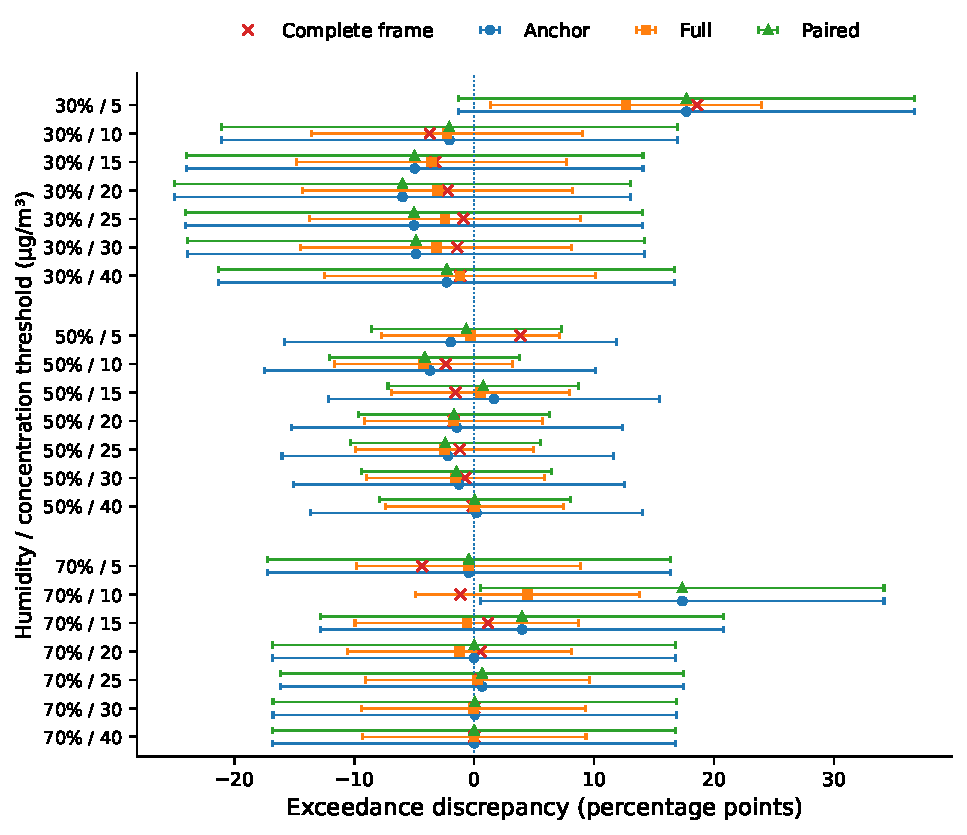
\includegraphics[width=\linewidth]{v2/figure5_epa_intervals.pdf}
\caption{Actual simultaneous limits in the first retained random-audit mask at the 20\% budget (369 unique references). All three humidity targets and seven thresholds are shown. Horizontal bars are limits for each method; crosses mark complete-frame values. Paired weights are $(0,0.8,0)$ at $(30,50,70)\%$ humidity. Repeated-mask coverage is reported in Table 3 of the main manuscript.}\label{fig:epa_intervals}
\noindent Alt text: Paired coincides with Anchor at 30 and 70 percent humidity and is narrower at 50 percent. One 70-percent interval misses its complete-frame value.
\end{figure}

\section{Weak-signal information boundary}
Let $S\in\{-1,1\}$ equally likely, $\Pr_\theta(Z=1\mid S)=1/2+\theta S$, $|\theta|<1/4$, and $R\sim\operatorname{Bernoulli}(p)$ independently. The augmentation path is $a_\lambda=1/2+\lambda dS$, $0<d<1/4$. Conditioning on $(S,Z)$ gives $\E U_\lambda=1/2$.

Write $V=Z-1/2$, so $\E V^2=1/4$ and $\E SV=\theta$. The centred augmented signal is $R V/p+(1-R/p)\lambda dS$. Expanding its square gives
\[
 p\Var(U_\lambda)=\tfrac14+(1-p)(d^2\lambda^2-2d\theta\lambda).
\]
For $p<1$ and $\theta\leq0$, every positive weight increases variance. For $0<\theta<d$, the optimum is $\lambda^\star=\theta/d$ and
\[
 g_\theta^\star=z_{1-\alpha/2}\left\{\tfrac12-
 \sqrt{\tfrac14-(1-p)\theta^2}\right\}
 =z_{1-\alpha/2}(1-p)\theta^2+O(\theta^4).
\]
The expansion is uniform for $p$ bounded away from one. At $p=1$ all augmentation corrections are zero and no gain exists.

The observed laws of $(S,R)$ coincide under $\theta$ and zero. Conditional on $R=1$, the Bernoulli relative entropy to success probability $1/2$ is at most its chi-squared divergence $4\theta^2$. Thus
\[
 \operatorname{KL}(P_\theta^{n_G},P_0^{n_G})\leq4n_Gp\theta^2.
\]
Pinsker's inequality gives total variation at most $\sqrt{2n_Gp}|\theta|$. For any event $A$ with $P_0(A)\leq\delta$,
\[
 P_\theta(A)\leq\delta+\sqrt{2n_Gp}|\theta|.
\]
To obtain a local model, take an independent $X$ and let the association be $\theta$ only within the box-kernel neighbourhood. If its probability is $r_h$, each observation contributes at most $4pr_h\theta^2$ to divergence. The effective information is therefore $n_Gpr_h\asymp n_Gph^d$. All unverified covariate and surrogate distributions agree across the alternatives.

For the converse certificate, conditional on $k$ verified observations, each $S_i(2Z_i-1)/2$ lies in $[-1/2,1/2]$ with mean $\theta$. Hoeffding's one-sided inequality implies $\Pr(\theta_L>\theta)\leq\delta$. On the complementary event, a positive chosen weight satisfies $0<d\widehat\lambda\leq\theta_L\leq\theta$. Consequently
\[
 p\Var(U_{\widehat\lambda})-p\Var(U_0)
 =(1-p)d\widehat\lambda(d\widehat\lambda-2\theta)
 \leq-(1-p)(d\widehat\lambda)^2<0.
\]
Another one-sided Hoeffding bound gives adoption probability at least $1-\beta$ under the signal inequality in the main theorem. Intersecting adoption with the valid lower-bound event gives probability at least $1-\beta-\delta$ of positive, beneficial borrowing. For $k=0$ use zero borrowing. This establishes matching fixed-submodel signal orders $k^{-1/2}$ and corresponding squared critical-gain order $k^{-1}$. Constants and multiplicity change with the requested confidence levels.

The target $P_\theta(Z=1)=1/2$ is constant in this submodel. Its role is to distinguish information needed to certify a variance reduction from information needed to estimate an otherwise known target; it is not a minimax lower bound for estimating $F_h$ across a general nonparametric model. The exact binomial enumeration in the reproduction code computes the certificate's adoption and harmful-selection probabilities without simulation error.

\section{Reference efficiency and extensions of the original framework}
\subsection{Canonical gradient and covariance excess}
For fixed $h$ and verification law, let $m_{0,y}(W)=\E(Z_y\mid W)$ and $F_h(y)=\E(K_hZ_y)/\mu_h$. The canonical gradient is
\begin{equation}\label{eq:efficient}
 \phi^{\mathrm{eff}}_{h,y}(O)=\frac{K_h}{\mu_h}
 \left\{m_{0,y}(W)+\frac R\pi(Z_y-m_{0,y}(W))-F_h(y)\right\}.
\end{equation}
To verify the gradient identity, write an observed-data score as $s_W(W)+Rs_Y(Y,W)$, where $\E s_W=0$ and $\E(s_Y\mid W)=0$. The pathwise derivative of $F_h$ is
\[
 \mu_h^{-1}\E\{K_h(Z_y-F_h)(s_W+s_Y)\}.
\]
Taking the inner product of \eqref{eq:efficient} with the observed score yields exactly this derivative, by iterated expectation and $\E R\mid W=\pi$. The displayed gradient lies in the observed tangent space: its first component is a mean-zero function of $W$, and its second is $R$ times a conditionally mean-zero residual. If the verification law is unknown, its additional tangent scores have form $(R-\pi)b(W)$; their inner products with \eqref{eq:efficient} vanish. Thus the same efficiency bound applies. This is the standard missing-data tangent-space argument specialised to the local distribution \citep{Tsiatis2006,RobinsRotnitzkyZhao1994}.

For any fixed augmentation $a$, write $\delta_y^a=a_y-m_{0,y}$ and $C_{yz}(W)=\Cov(Z_y,Z_z\mid W)$. Then
\[
 U_y(a)=m_{0,y}+\frac R\pi(Z_y-m_{0,y})+(1-R/\pi)\delta_y^a.
\]
Conditional cross-covariances between the two residual terms are zero because $\E(Z_y-m_{0,y}\mid W)=0$. Therefore
\begin{equation}
 \Cov\{U_y(a),U_z(a)\mid W\}
 =\frac{C_{yz}(W)}{\pi(W)}+(\pi(W)^{-1}-1)\delta_y^a\delta_z^a.
\end{equation}
The conditional means are $m_{0,y}$. Taking total covariance and multiplying by the kernel factors shows that the influence covariance exceeds the efficient one by
\begin{equation}\label{eq:excess}
 \mu_h^{-2}\E\{K_h^2(\pi^{-1}-1)\delta_y^a\delta_z^a\}.
\end{equation}
Over every finite grid this is positive semidefinite. If an estimator attains the true $m_0$, it dominates other fixed augmentations in covariance and in centred convex Gaussian-set probabilities. The fitted scalar path in the separation example need not contain that estimator; this is why the example does not conflict with operator-efficiency results such as \citet{zhang2026generation}.

\subsection{The integrated-variance rule as a comparison method}
Put $A=m_0-q$, $D=m-q$, and use a finite threshold measure $\nu$. The augmentation-dependent integrated variance is
\[
 J_h(\lambda)=\E\{v_h^*(W)\|A-\lambda D\|_\nu^2\},\quad
 v_h^*(W)=\frac{h^dK_h^2}{\mu_h^2}(\pi^{-1}-1).
\]
Direct expansion gives $J_h(\lambda)=J_h(0)-2\lambda G_h+\lambda^2H_h$, where
\[
 G_h=\E\{v_h^*\langle A,D\rangle_\nu\},\qquad
 H_h=\E\{v_h^*\|D\|_\nu^2\}.
\]
Since $\E\{R\pi^{-1}(Z-q)\mid W\}=A$, $G_h$ has an observable inverse-probability representation. For $H_h>0$ the constrained optimum is $\Pi_{[0,1]}(G_h/H_h)$; for $H_h=0$ use zero. Full borrowing improves the anchor exactly when $2G_h-H_h>0$. The improvement is zero when $G_h\leq0$, $G_h^2/H_h$ when $0<G_h<H_h$, and $2G_h-H_h$ when $G_h\geq H_h>0$.

These are retained as efficiency identities and motivate the Trace comparator; they are not counted as new paired-certification principles. Covariance-based trace estimation in the new simulation targets the trace of the full fitted-path covariance, including all terms independent of the weight. Its population minimiser agrees with the equal-weight version of the integrated criterion.

For the earlier ratio selector, bounded moments give normalised estimates $p(\widehat G_h-G_h),p(\widehat H_h-H_h)=O_P(N_G^{-1/2})$. If $pH_h$ is bounded below, the projection map and a ratio expansion imply $\widehat\lambda-\lambda^{\mathrm{or}}=O_P(N_G^{-1/2})$. The correction in an independent evaluation mean has variance of order $(\widehat\lambda-\lambda^{\mathrm{or}})^2$ on the local process scale; it is therefore $o_P(1)$. If the correction collapses in the uniform local verification norm, every bounded difference of weights has the same negligible evaluation effect. With an entropy bound this argument extends from finite thresholds to the whole process. It does not require treating a random fitted regression as the true conditional distribution.

\subsection{Local covariance limit and point-target bias}
Suppose $h\to0$, $p\to p_\infty\in[0,1]$, $e(W)$ converges locally to $e_0(W)$, and the fitted limiting augmentation is $a_\infty$. Write $\delta=a_\infty-m_0$. Kernel change of variables, uniform local covariance convergence and dominated convergence give the covariance of the $\sqrt{nph^d}$-scaled ratio process:
\begin{align}
 \Gamma(y,z)=\frac{\kappa_K}{f_X(x_0)}\E\big[&C_{yz}/e_0+(e_0^{-1}-p_\infty)\delta_y\delta_z\notag\\
 &+p_\infty\{m_{0,y}-F_0(y\mid x_0)\}\{m_{0,z}-F_0(z\mid x_0)\}\mid X=x_0\big],
\end{align}
where $\kappa_K=\int K^2/(\int K)^2$. To see the normalisation, write $\mu_h=h^df_X(x_0)\int K+o(h^d)$ and
$\E K_h^2b(W)=h^df_X(x_0)\int K^2\E\{b(W)\mid X=x_0\}+o(h^d)$.
The three terms follow from conditional covariance plus covariance of the conditional mean. Verification scarcity affects the rate and removes the last term when $p_\infty=0$; selective allocation remains through $e_0^{-1}$.

For a symmetric second-order kernel, a twice differentiable covariate density and conditional distribution with uniformly bounded second derivatives,
\[
 \E K_hZ_y=h^d\int K(u)F_0(y\mid x_0+hu)f_X(x_0+hu)\,du.
\]
Taylor expansion makes first-order terms vanish by symmetry. Expanding the denominator in the same way yields $\sup_y|F_h(y)-F_0(y\mid x_0)|=O(h^2)$. Hence $\sqrt{nph^d}h^2\to0$ transfers the centred process limit and band to the point target. A bias-corrected alternative must also estimate and include the variability of its correction.

If $F_0$ is strictly increasing and has continuous density bounded away from zero on the quantile range, an ordinary inverse-map expansion gives
\[
 \sqrt{nph^d}(\widehat Q(\tau)-Q_0(\tau))
 =-\frac{\sqrt{nph^d}\{\widehat F(Q_0(\tau))-F_0(Q_0(\tau))\}}
 {f_{Y\mid X}(Q_0(\tau)\mid x_0)}+o_P(1)
\]
uniformly in an interior compact probability interval. Rearrangement is first-order neutral under these strict-monotonicity conditions \citep{ChernozhukovEtAl2010}. At atoms, use band inversion from S4 rather than this density formula.

\subsection{Estimated verification probabilities}
For a separately fitted $\widehat\pi$ and a fixed candidate $a$, the exact conditional drift is
\begin{equation}
 \E\left[a+\frac R{\widehat\pi}(Z-a)-Z\,\middle|\,W\right]
 =\frac{\widehat\pi-\pi}{\widehat\pi}(a-m_0).
\end{equation}
For local normalised averaging, put
\[
 r_\pi^2=\mu_h^{-1}\E\left[K_h
 \left\{(\widehat\pi-\pi)/\widehat\pi\right\}^2\right],\qquad
 r_a^2=\mu_h^{-1}\E[K_h(a-m_0)^2].
\]
Cauchy--Schwarz bounds the local drift by $r_\pi r_a$. A sufficient bias condition for pointwise inference is $\sqrt{nph^d}r_\pi r_a=o_P(1)$, uniformly over the reported thresholds. The empirical-process replacement additionally requires the local weighted second moment of the signal difference to vanish, for example
\[
 \frac{ph^d}{\mu_h^2}\E\left[K_h^2\pi
 \{\widehat\pi^{-1}-\pi^{-1}\}^2(Z-a)^2\right]=o_P(1),
\]
with an appropriate entropy condition for uniform inference. Positivity bounds must hold for $\widehat\pi/\pi$. A learned propensity also affects covariance-slope calibration, requiring its estimated influence or a nuisance remainder negligible on that calibration scale. The primary simulations and EPA analysis use known probabilities. The training-fold logistic sensitivity in Section S10 additionally measures plug-in performance; it does not treat propensity-model correctness alone as proof of the required drift and calibration-score conditions.

\subsection{Local linear estimation and verification allocation}
A local linear alternative uses $V_h=(1,(X-x_0)^\top/h)^\top$, $Q_h=\E K_hV_hV_h^\top$ and
$\beta_h(y)=Q_h^{-1}\E K_hV_hZ_y$. Its intercept influence for fixed $h$ is
\[
 e_1^\top Q_h^{-1}K_hV_h\{U_y(a)-V_h^\top\beta_h(y)\}.
\]
This follows by differentiating the weighted normal equation; the derivative of $Q_h^{-1}$ supplies the fitted-linear-term subtraction. The same joint path-covariance and paired-gain construction applies when $Q_h$ is nonsingular. Local linear equivalent weights can be negative, so the finite-resolution intercept need not be a cumulative distribution. Monotone whole-distribution envelopes apply to the point target only after the appropriate localisation-bias control establishes grid coverage for that target.

Finally, for an augmentation fixed independently of the audit design, the part of an integrated variance depending on the verification law is of the form $\E[A(W)/\pi(W)]$, $A\geq0$. Under $\E\pi=p$, Cauchy--Schwarz gives
$\E[A/\pi]\geq\{\E\sqrt A\}^2/p$, with equality at $\pi\propto\sqrt A$ when unconstrained. Under lower and upper probability bounds the pointwise Karush--Kuhn--Tucker equation gives the clipped square-root allocation, with its constant chosen to satisfy the budget. This is an allocation extension of the original variance criterion, not an assertion that it minimises a simultaneous critical value. The present work fixes the known verification design and certifies borrowing conditional on that design.

\section{Reproduction, numerical diagnostics and complete results}
\subsection{Frozen protocols and provenance}
The source archive is pinned to commit \texttt{70c47c5}; the complete identifier is recorded in the source manifest. The date mapping was transferred losslessly: its 43,937 bytes have Git blob hash \texttt{aaab1595ce2f0848783ff4015009ac6218caf5d3}. The reconstructed analysis table preserves all 2,814 supplied observation identifiers, concentrations and humidities. Joining the mapping produces no missing dates or duplicate station--date pairs. The recovery script supplied by the authors checked the three numerical columns and station identity against the archived RDS before extracting its dates. The reproduction package records these source checks separately from the new analyses.

The revised primary simulation contains 6,000 independently generated replications and 36,000 method-level records. Every replication ran successfully; no failed-information fallback occurred in the primary grid. The code keeps the earlier exploratory simulation in \texttt{results/prior\_checkpoint}; it is not pooled with the guarded simulation. New results reside in \texttt{results/guarded\_main}. The exact binary calculations and original technical note are retained with their own provenance.

The simulation verification law is random or
\[
 \pi(x,s)=p\left[1+0.4\tanh\left\{
 \frac{s-\ell(x)\mu(x)}{\sqrt{\ell(x)^2\sigma(x)^2+\tau^2}}
 \right\}\right].
\]
The conditional standardised surrogate has a symmetric distribution, so this design has mean $p$ without using reference outcomes to calibrate the probability. Mean regression uses $1,x,x^2$ for the anchor and adds $s$ for the surrogate candidate; residual standard deviation is estimated within the training role. The anchor fit uses inverse-probability weights and the surrogate fit uses equal weights. Their outputs are bounded Gaussian distribution predictions even under misspecification. The matrix-projection comparator uses the stated fixed relative ridge and is not restricted to the scalar path.

All reported primary bands cover the raw estimator on the declared grid. Integrated squared error is also computed for this raw grid estimator. This differs from earlier archived comparisons of rearranged point estimates. The inferential and risk targets are recorded in the manifest, rather than inferred from a figure label.

\subsection{Numerical accuracy and software checks}
The radial Gaussian derivative is checked by central finite differences in dimensions one, two and five. The largest relative discrepancy is below $6\times10^{-10}$. The two-threshold separation calculation is compared against deterministic Gaussian rectangle integration; the largest discrepancy in the four tested critical values is below $9\times10^{-7}$. An independent perturbation of the empirical distribution verifies the covariance-centring influence term to absolute error below $7\times10^{-11}$.

The new numerical audit compares 8,192 and 32,768 radial directions in 60 fitted-data replications. All 60 paired selections agree. The largest change in a radial critical value is $3.935\times10^{-4}$; the largest change in a paired radial gain is $4.475\times10^{-4}$. Refining population-covariance integration from 48 by 24 quadrature points to 96 by 64 changes a covariance entry by at most $2.662\times10^{-5}$. These are deterministic refinement checks on the evaluated cases. The fresh Gaussian order-statistic intervals, not these observed differences, provide the numerical probability guarantees used by the selector.

Thirty additional revision checks verify date provenance, historical/audit separation, concentration reconstruction, exact binomial quantile ranks, positive-semidefinite covariance handling, the unique-reference budget identity, exact finite-frame covariance enumeration, unbiased gate moments, gate-score variance and whole-distribution envelopes at atoms. Hidden reference outcomes are changed while keeping all visible variables and masks fixed; the EPA selected weights, point estimates and confidence limits remain unchanged. The code treats materially negative eigenvalues as an error and clips only negative values within its stated floating-point tolerance. All checks pass.

An observed zero harmful-selection count is not a probability guarantee. For zero events in 500 independent replications, the exact two-sided 95\% binomial upper limit is approximately $0.00735$; the one-sided 95\% upper limit is approximately $0.00597$. Machine-readable exact intervals accompany every simulation coverage and numerical-harm entry. The primary harm threshold is $10^{-4}$ in the normalised population Gaussian critical value, and the quadrature audit quantifies, but does not rigorously bound, its residual assessment error.

\subsection{Three-role rotation}
A separate 400-replication experiment allocates error across three role-specific bands. Each evaluation role uses Gaussian tail probability $0.047/3$ plus numerical error $0.001$, for a total no greater than $0.05$ across rotations. Gate certificates allocate $0.047/3$ to statistical calibration and $0.001$ to the two numerical events. There are 200 aligned and 200 locally reversed replications.

In the aligned design, the intersection band has coverage $0.960$ for Anchor and $0.970$ for Paired, with mean widths $0.264$ and $0.202$. Under local reversal both methods have coverage $0.975$ and mean width $0.263$. No empty intersections occur. Convex aggregation covers in every observed replication and is wider: aligned widths are $0.358$ and $0.273$, respectively. These results illustrate the price of dependence-valid rotation without relying on a pooled Gaussian approximation for jointly selected role estimates.

\subsection{EPA decisions and reference support}
The six EPA design--budget combinations contain 1,200 audit masks and 18,000 method--target records, with no computation failures. The complete audit frame is held fixed. Monte Carlo coverage variation is therefore variation over designed reference selection, not environmental population sampling.

At $30\%$ humidity and concentration 5, the complete-frame exceedance discrepancy is $18.602$ percentage points. Under random auditing, Paired's simultaneous interval resolves its positive sign in $1.0\%$, $9.5\%$ and $68.0\%$ of masks at the 5\%, 10\% and 20\% budgets. At concentration 15 the smaller upper-tail differences are generally unresolved: at the 20\% random budget, the resolution rates are $0\%$, $0.5\%$ and $0\%$ at the three humidity targets. This separates a precise description available with all reference measurements from what a sparse audit can establish. It does not convert absence of a resolved sign into evidence of exact calibration.

All pointwise decisions are recovered from the retained selected weights, evaluation widths and reference-mask seeds, without rerunning a selector or choosing new thresholds. Their reconstructed estimates and limits match the stored example bands to floating-point precision. The resulting 126,000 pointwise records and all sign-resolution summaries are retained in the code archive. For an evaluation neighbourhood with fewer than three reference values, the procedure reports the full feasible distribution band translated by the known sensor distribution; all such cases are explicitly flagged.

The next two tables provide every main simulation and EPA comparison. Monte Carlo standard errors for additional metrics and exact binomial intervals are in the machine-readable tables. The full-reference legacy VitalDB and controlled synthetic review results remain in the original project archive; they are not represented as evaluations of the new paired selector.
\begingroup\setlength{\tabcolsep}{4pt}
\begin{longtable}{rlrrrrr}
\caption{Complete primary simulation comparisons: 500 replications per method and cell.}\label{tab:allsim}\\
\toprule
Cell & Method & Coverage & MCSE & Width ratio & Harm & Adoption\\
\midrule
\endfirsthead
\toprule
Cell & Method & Coverage & MCSE & Width ratio & Harm & Adoption\\
\midrule
\endhead
\bottomrule\endfoot
1 & Anchor & 0.958 & 0.009 & 1.000 & 0.000 & 0.000\\
1 & Full & 0.958 & 0.009 & 0.722 & 0.000 & 1.000\\
1 & Paired & 0.954 & 0.009 & 0.803 & 0.000 & 0.862\\
1 & Plug-in & 0.960 & 0.009 & 0.723 & 0.000 & 1.000\\
1 & Projection & 0.956 & 0.009 & 0.750 & 0.000 & --\\
1 & Trace & 0.960 & 0.009 & 0.721 & 0.000 & 1.000\\
2 & Anchor & 0.956 & 0.009 & 1.000 & 0.000 & 0.000\\
2 & Full & 0.960 & 0.009 & 0.722 & 0.000 & 1.000\\
2 & Paired & 0.956 & 0.009 & 0.747 & 0.000 & 1.000\\
2 & Plug-in & 0.962 & 0.009 & 0.723 & 0.000 & 1.000\\
2 & Projection & 0.958 & 0.009 & 0.734 & 0.000 & --\\
2 & Trace & 0.962 & 0.009 & 0.722 & 0.000 & 1.000\\
3 & Anchor & 0.962 & 0.009 & 1.000 & 0.000 & 0.000\\
3 & Full & 0.956 & 0.009 & 0.759 & 0.000 & 1.000\\
3 & Paired & 0.958 & 0.009 & 0.769 & 0.000 & 1.000\\
3 & Plug-in & 0.954 & 0.009 & 0.759 & 0.000 & 1.000\\
3 & Projection & 0.966 & 0.008 & 0.764 & 0.000 & --\\
3 & Trace & 0.954 & 0.009 & 0.759 & 0.000 & 1.000\\
4 & Anchor & 0.952 & 0.010 & 1.000 & 0.000 & 0.000\\
4 & Full & 0.966 & 0.008 & 0.723 & 0.000 & 1.000\\
4 & Paired & 0.956 & 0.009 & 0.831 & 0.000 & 0.752\\
4 & Plug-in & 0.968 & 0.008 & 0.724 & 0.000 & 1.000\\
4 & Projection & 0.980 & 0.006 & 0.761 & 0.000 & --\\
4 & Trace & 0.970 & 0.008 & 0.722 & 0.000 & 1.000\\
5 & Anchor & 0.936 & 0.011 & 1.000 & 0.000 & 0.000\\
5 & Full & 0.958 & 0.009 & 0.715 & 0.000 & 1.000\\
5 & Paired & 0.952 & 0.010 & 0.750 & 0.000 & 0.994\\
5 & Plug-in & 0.956 & 0.009 & 0.715 & 0.000 & 1.000\\
5 & Projection & 0.966 & 0.008 & 0.733 & 0.000 & --\\
5 & Trace & 0.956 & 0.009 & 0.714 & 0.000 & 1.000\\
6 & Anchor & 0.970 & 0.008 & 1.000 & 0.000 & 0.000\\
6 & Full & 0.958 & 0.009 & 0.738 & 0.000 & 1.000\\
6 & Paired & 0.962 & 0.009 & 0.755 & 0.000 & 1.000\\
6 & Plug-in & 0.958 & 0.009 & 0.739 & 0.000 & 1.000\\
6 & Projection & 0.958 & 0.009 & 0.746 & 0.000 & --\\
6 & Trace & 0.960 & 0.009 & 0.739 & 0.000 & 1.000\\
7 & Anchor & 0.960 & 0.009 & 1.000 & 0.000 & 0.000\\
7 & Full & 0.966 & 0.008 & 0.954 & 0.000 & 1.000\\
7 & Paired & 0.960 & 0.009 & 1.000 & 0.000 & 0.000\\
7 & Plug-in & 0.962 & 0.009 & 0.955 & 0.000 & 0.998\\
7 & Projection & 0.960 & 0.009 & 0.966 & 0.014 & --\\
7 & Trace & 0.964 & 0.008 & 0.955 & 0.000 & 1.000\\
8 & Anchor & 0.954 & 0.009 & 1.000 & 0.000 & 0.000\\
8 & Full & 0.958 & 0.009 & 1.114 & 0.994 & 1.000\\
8 & Paired & 0.954 & 0.009 & 1.000 & 0.000 & 0.000\\
8 & Plug-in & 0.954 & 0.009 & 1.000 & 0.000 & 0.006\\
8 & Projection & 0.966 & 0.008 & 0.805 & 0.000 & --\\
8 & Trace & 0.954 & 0.009 & 1.000 & 0.000 & 0.006\\
9 & Anchor & 0.968 & 0.008 & 1.000 & 0.000 & 0.000\\
9 & Full & 0.968 & 0.008 & 1.001 & 0.694 & 1.000\\
9 & Paired & 0.968 & 0.008 & 1.000 & 0.000 & 0.000\\
9 & Plug-in & 0.966 & 0.008 & 1.000 & 0.312 & 0.476\\
9 & Projection & 0.958 & 0.009 & 1.013 & 1.000 & --\\
9 & Trace & 0.966 & 0.008 & 1.000 & 0.310 & 0.492\\
10 & Anchor & 0.944 & 0.010 & 1.000 & 0.000 & 0.000\\
10 & Full & 0.944 & 0.010 & 1.000 & 0.000 & 1.000\\
10 & Paired & 0.944 & 0.010 & 1.000 & 0.000 & 0.000\\
10 & Plug-in & 0.944 & 0.010 & 1.000 & 0.000 & 0.000\\
10 & Projection & 0.944 & 0.010 & 1.000 & 0.000 & --\\
10 & Trace & 0.944 & 0.010 & 1.000 & 0.000 & 0.000\\
11 & Anchor & 0.958 & 0.009 & 1.000 & 0.000 & 0.000\\
11 & Full & 0.964 & 0.008 & 0.721 & 0.000 & 1.000\\
11 & Paired & 0.968 & 0.008 & 0.731 & 0.000 & 1.000\\
11 & Plug-in & 0.966 & 0.008 & 0.721 & 0.000 & 1.000\\
11 & Projection & 0.966 & 0.008 & 0.727 & 0.000 & --\\
11 & Trace & 0.966 & 0.008 & 0.721 & 0.000 & 1.000\\
12 & Anchor & 0.956 & 0.009 & 1.000 & 0.000 & 0.000\\
12 & Full & 0.954 & 0.009 & 1.135 & 1.000 & 1.000\\
12 & Paired & 0.956 & 0.009 & 1.000 & 0.000 & 0.000\\
12 & Plug-in & 0.956 & 0.009 & 1.000 & 0.002 & 0.002\\
12 & Projection & 0.954 & 0.009 & 0.839 & 0.004 & --\\
12 & Trace & 0.956 & 0.009 & 1.000 & 0.002 & 0.002\\
\end{longtable}\endgroup
\begingroup\setlength{\tabcolsep}{4pt}
\begin{longtable}{rrlrrrr}
\caption{Targetwise EPA design-based performance. R and S denote random and selective audit; the following number is the budget percentage.}\label{tab:allepa}\\
\toprule
Design & RH & Method & Coverage & Width ratio & Weight & Harm\\
\midrule
\endfirsthead
\toprule
Design & RH & Method & Coverage & Width ratio & Weight & Harm\\
\midrule
\endhead
\bottomrule\endfoot
R5 & 30 & Anchor & 0.985 & 1.000 & 0.000 & 0.000\\
R5 & 30 & Full & 0.995 & 0.653 & 1.000 & 0.000\\
R5 & 30 & Paired & 0.985 & 0.996 & 0.011 & 0.000\\
R5 & 30 & Plug-in & 0.995 & 0.676 & 0.897 & 0.000\\
R5 & 30 & Trace & 0.995 & 0.663 & 0.947 & 0.000\\
R5 & 50 & Anchor & 0.980 & 1.000 & 0.000 & 0.000\\
R5 & 50 & Full & 0.995 & 0.690 & 1.000 & 0.000\\
R5 & 50 & Paired & 0.980 & 0.975 & 0.072 & 0.000\\
R5 & 50 & Plug-in & 0.995 & 0.699 & 0.882 & 0.000\\
R5 & 50 & Trace & 0.995 & 0.695 & 0.919 & 0.000\\
R5 & 70 & Anchor & 0.990 & 1.000 & 0.000 & 0.000\\
R5 & 70 & Full & 1.000 & 0.694 & 1.000 & 0.000\\
R5 & 70 & Paired & 0.990 & 0.985 & 0.048 & 0.000\\
R5 & 70 & Plug-in & 1.000 & 0.712 & 0.865 & 0.000\\
R5 & 70 & Trace & 1.000 & 0.702 & 0.912 & 0.000\\
R10 & 30 & Anchor & 0.985 & 1.000 & 0.000 & 0.000\\
R10 & 30 & Full & 0.990 & 0.646 & 1.000 & 0.000\\
R10 & 30 & Paired & 0.990 & 0.980 & 0.051 & 0.000\\
R10 & 30 & Plug-in & 0.990 & 0.657 & 0.927 & 0.000\\
R10 & 30 & Trace & 0.990 & 0.649 & 0.972 & 0.000\\
R10 & 50 & Anchor & 0.980 & 1.000 & 0.000 & 0.000\\
R10 & 50 & Full & 0.990 & 0.678 & 1.000 & 0.000\\
R10 & 50 & Paired & 0.980 & 0.899 & 0.226 & 0.000\\
R10 & 50 & Plug-in & 0.990 & 0.682 & 0.902 & 0.000\\
R10 & 50 & Trace & 0.990 & 0.679 & 0.934 & 0.000\\
R10 & 70 & Anchor & 0.990 & 1.000 & 0.000 & 0.000\\
R10 & 70 & Full & 0.990 & 0.677 & 1.000 & 0.000\\
R10 & 70 & Paired & 0.990 & 0.948 & 0.134 & 0.000\\
R10 & 70 & Plug-in & 0.990 & 0.684 & 0.906 & 0.000\\
R10 & 70 & Trace & 0.985 & 0.679 & 0.933 & 0.000\\
R20 & 30 & Anchor & 0.990 & 1.000 & 0.000 & 0.000\\
R20 & 30 & Full & 0.995 & 0.637 & 1.000 & 0.000\\
R20 & 30 & Paired & 0.985 & 0.872 & 0.302 & 0.000\\
R20 & 30 & Plug-in & 0.990 & 0.644 & 0.955 & 0.000\\
R20 & 30 & Trace & 0.995 & 0.638 & 0.987 & 0.000\\
R20 & 50 & Anchor & 0.990 & 1.000 & 0.000 & 0.000\\
R20 & 50 & Full & 1.000 & 0.670 & 1.000 & 0.000\\
R20 & 50 & Paired & 0.995 & 0.758 & 0.559 & 0.000\\
R20 & 50 & Plug-in & 1.000 & 0.672 & 0.926 & 0.000\\
R20 & 50 & Trace & 1.000 & 0.670 & 0.959 & 0.000\\
R20 & 70 & Anchor & 0.990 & 1.000 & 0.000 & 0.000\\
R20 & 70 & Full & 0.980 & 0.671 & 1.000 & 0.000\\
R20 & 70 & Paired & 0.990 & 0.855 & 0.349 & 0.000\\
R20 & 70 & Plug-in & 0.980 & 0.673 & 0.943 & 0.000\\
R20 & 70 & Trace & 0.980 & 0.672 & 0.951 & 0.000\\
S5 & 30 & Anchor & 0.965 & 1.000 & 0.000 & 0.000\\
S5 & 30 & Full & 1.000 & 0.676 & 1.000 & 0.000\\
S5 & 30 & Paired & 0.965 & 1.000 & 0.000 & 0.000\\
S5 & 30 & Plug-in & 0.990 & 0.696 & 0.876 & 0.000\\
S5 & 30 & Trace & 0.985 & 0.683 & 0.925 & 0.000\\
S5 & 50 & Anchor & 0.990 & 1.000 & 0.000 & 0.000\\
S5 & 50 & Full & 0.995 & 0.671 & 1.000 & 0.000\\
S5 & 50 & Paired & 0.990 & 0.967 & 0.077 & 0.000\\
S5 & 50 & Plug-in & 0.995 & 0.682 & 0.895 & 0.000\\
S5 & 50 & Trace & 0.995 & 0.678 & 0.927 & 0.000\\
S5 & 70 & Anchor & 1.000 & 1.000 & 0.000 & 0.000\\
S5 & 70 & Full & 0.995 & 0.647 & 1.000 & 0.000\\
S5 & 70 & Paired & 1.000 & 0.998 & 0.013 & 0.000\\
S5 & 70 & Plug-in & 0.995 & 0.669 & 0.864 & 0.000\\
S5 & 70 & Trace & 0.995 & 0.656 & 0.921 & 0.000\\
S10 & 30 & Anchor & 0.960 & 1.000 & 0.000 & 0.000\\
S10 & 30 & Full & 0.990 & 0.649 & 1.000 & 0.000\\
S10 & 30 & Paired & 0.960 & 0.994 & 0.011 & 0.000\\
S10 & 30 & Plug-in & 0.990 & 0.668 & 0.915 & 0.000\\
S10 & 30 & Trace & 0.990 & 0.654 & 0.960 & 0.000\\
S10 & 50 & Anchor & 0.980 & 1.000 & 0.000 & 0.000\\
S10 & 50 & Full & 0.995 & 0.651 & 1.000 & 0.000\\
S10 & 50 & Paired & 0.980 & 0.890 & 0.234 & 0.000\\
S10 & 50 & Plug-in & 0.995 & 0.657 & 0.908 & 0.000\\
S10 & 50 & Trace & 0.995 & 0.655 & 0.937 & 0.000\\
S10 & 70 & Anchor & 0.985 & 1.000 & 0.000 & 0.000\\
S10 & 70 & Full & 0.995 & 0.656 & 1.000 & 0.000\\
S10 & 70 & Paired & 0.985 & 0.966 & 0.070 & 0.000\\
S10 & 70 & Plug-in & 0.995 & 0.661 & 0.901 & 0.000\\
S10 & 70 & Trace & 0.995 & 0.656 & 0.932 & 0.000\\
S20 & 30 & Anchor & 0.975 & 1.000 & 0.000 & 0.000\\
S20 & 30 & Full & 0.990 & 0.647 & 1.000 & 0.000\\
S20 & 30 & Paired & 0.975 & 0.935 & 0.166 & 0.000\\
S20 & 30 & Plug-in & 0.985 & 0.663 & 0.930 & 0.000\\
S20 & 30 & Trace & 0.985 & 0.652 & 0.970 & 0.000\\
S20 & 50 & Anchor & 0.985 & 1.000 & 0.000 & 0.000\\
S20 & 50 & Full & 1.000 & 0.646 & 1.000 & 0.000\\
S20 & 50 & Paired & 0.985 & 0.746 & 0.558 & 0.000\\
S20 & 50 & Plug-in & 1.000 & 0.649 & 0.939 & 0.000\\
S20 & 50 & Trace & 1.000 & 0.647 & 0.962 & 0.000\\
S20 & 70 & Anchor & 0.995 & 1.000 & 0.000 & 0.000\\
S20 & 70 & Full & 0.995 & 0.652 & 1.000 & 0.000\\
S20 & 70 & Paired & 0.995 & 0.888 & 0.240 & 0.000\\
S20 & 70 & Plug-in & 0.990 & 0.654 & 0.923 & 0.000\\
S20 & 70 & Trace & 0.990 & 0.652 & 0.947 & 0.000\\
\end{longtable}\endgroup

\section{Dense thresholds, matched certification and precision requirements}\label{sec:s10}
\subsection{Experiments fixed before the additional runs}
The additional protocol contains three modules: six pairing-ablation cells with 500 replications each, six dense-grid cells with 200 replications each, and seven robustness cells with 300 replications each. This gives 6,300 design--grid replications and 37,800 method records. The dense-grid cells deliberately reuse each generated dataset at three grid resolutions: they contain 400 distinct datasets, not 1,200 independent datasets. The additional modules together use 5,500 distinct generated datasets. All six methods within a replication share training, reference masks, gate and evaluation data. These runs are separate from the 6,000 primary replications.

The ablation repeats alignment at reference fractions $0.05,0.10,0.20$ and weak, reversed and absent signals at fraction $0.10$, always with $n=6,000$, $h=0.35$ and seven thresholds. Unpaired uses the absolute-critical-value bounds of Section S3.5, with statistical errors $0.0245$ for the anchor and for the candidate maximum. The two upper simulated quantiles each receive error $0.00025$. Its Gaussian numerical intervals are exactly the same intervals used by Paired and have total error $0.0005$. Thus each selector has total statistical-plus-numerical error $0.05$. Each absolute Taylor expansion receives the same $b_N$ cushion; the sum is $2b_N$, compared with Paired's $\lambda b_N$. This is part of the error-cancellation comparison, not a different reference budget. The other four methods are Anchor, Full, Trace and Plug-in. The matrix Projection comparator remains in the primary experiment.

The dense experiments use $J=21,51,101$ thresholds $0.8\Phi^{-1}(u_j)$ with evenly spaced $u_j\in[0.02,0.98]$. The 21- and 51-point grids are subsets of the 101-point grid. Both alignment with random verification and local reversal with selective verification use $n=6,000$, $p=0.10$ and $h=0.35$. A common enlargement $10^{-8}I_J$ is declared for these calculations. Every reference mask, candidate regression and generated dataset is shared across grid resolutions. We evaluate the raw simultaneous band on its grid and its monotone envelope on a common 1,001-point grid. The latter is a numerical check of the envelope; the all-threshold guarantee follows from monotonicity as proved in Section S4. The experiment does not replace a growing-grid regularity condition by an empirical coverage estimate.

\subsection{Outcome and nuisance-regression robustness}
The three continuous non-Gaussian designs replace the normal error by a standardised $t_3$, $(\chi^2_3-3)/\sqrt6$, or $(A+0.5Z)/\sqrt{1.25}$ with independent $A\in\{-1,1\}$ equally likely and $Z\sim N(0,1)$. Mean and scale functions are unchanged. These errors have mean zero and variance one. Candidate Gaussian distribution regressions can be misspecified, while their threshold predictions remain bounded. Surrogate noise is Gaussian with standard deviation $0.4$.

For the ordinal design, generate the normal latent outcome and discretise it using nine cutpoints equally spaced from $-2$ to $2$, producing categories $0,\ldots,9$. Set $S=Y+0.4\eta$ and evaluate all nine nontrivial cumulative probabilities. True probabilities use the latent normal distribution at the category cutpoints. The two-dimensional design takes independent $X_1,X_2\sim U[-1,1]$, mean $1.2X_1+0.6X_1^2+0.8X_2$, scale $0.8+0.25(X_1^2+X_2^2)$, a product Epanechnikov kernel with $h=0.5$, and target $(0,0)$. Its local information is $n_Gph^2$.

A separate nonparametric-candidate design uses empirical neighbour distribution functions: the anchor searches in $X$, and the surrogate candidate in $(X,S)$. Coordinates are divided by their verified-training standard deviations, floored at $0.1$. The neighbour count is the smaller of the verified-training count and $\max\{20,\lfloor\sqrt{n_{T,R}}\rfloor\}$. All nine nontrivial category thresholds are used for the ordinal design; other robustness cells have 21 thresholds on the same probability range as the dense-grid study. All have $n=6,000$, $p=0.10$, and common enlargement $10^{-8}I_J$.

The learned-verification sensitivity uses
$\pi(X)=\operatorname{expit}(a+0.8X)$, with $a$ determined by $\E\pi(X)=0.10$. A logistic regression of $R$ on $(1,X)$ is fitted only in the training role; its predictions are clipped to $[0.005,0.5]$. These fitted probabilities replace the known design probabilities in the downstream signals. This cell measures actual plug-in sensitivity and is reported separately from the known-probability calibration result. Learned-probability inference requires the local drift and score-replacement conditions in Section S8; fitting a correct propensity model alone does not establish those product-rate conditions for every misspecified outcome regression.

For each design, the reference CDF is computed by integrating its known conditional distribution over the kernel neighbourhood, using 100-node Gauss--Legendre quadrature per covariate. Independent refinement to 180 nodes is checked. Population critical-value gains and harmful-selection probabilities are reported only in the normal, one-dimensional, Gaussian-candidate known-design cases where the conditional Gaussian covariance calculation applies. They are left unavailable in the other cells, rather than replacing an exact population comparison by an unlabelled finite truth sample. Coverage, width, distribution loss and adoption remain observed in every cell.

\subsection{Numerical refinement at dense thresholds}
The first five replication identifiers in each dense-grid cell are re-evaluated with 8,192 and 32,768 radial directions. These 30 comparisons were fixed before the refinement. Both calculations retain the same numerical critical-value intervals and total confidence budgets. We report changes in critical values, score radii, chosen weights, evaluation widths and point estimates. Weight agreement alone is not a measure of Gaussian integration accuracy when several grid choices have similar lower gains. The delivered records retain every disagreement and its inferential consequences. Independent directional finite differences also check the gradient in dimensions 21, 51 and 101. These calculations validate the implementation of the numerical derivative and measure integration sensitivity; the separate direct-Gaussian order-statistic construction supplies the numerical critical-value probability guarantee.

\subsection{Additional results and interpretation}
The completed run contains 6,300 design--grid replications, with no execution failures. Table~\ref{tab:s10-validation} gives coverage, width and adoption for every additional cell and method. Exact binomial intervals and Monte Carlo standard errors for all continuous summaries accompany the machine-readable table. These are cellwise Monte Carlo intervals, not a simultaneous assertion across all simulation cells. The dense output eigenvalues and local reference counts are retained alongside each replication. The 1,001-point envelope check is separate from grid coverage.

In the paired ablation, width differences and their standard errors are computed within the same generated sample. Two absolute critical-value bounds can remain too wide to certify a gain even when the paired difference can do so. The lower-bound constants and the allocation of error are fully disclosed in Section S3.5; this experiment isolates the stated implementations rather than every possible unpaired optimisation.

In the 30 dense refinement cases, 25 weights agree. Maximum absolute changes in radial critical values and paired radial gains are 0.005813 and 0.004265. Maximum relative changes in an evaluated band width and in the corresponding population critical value are 3.258\% and 2.140\%. No refined selected candidate in these cases has a negative assessed gain. Selection labels, integration error and inferential impact are therefore all recorded, rather than requiring equality of a mesh index as a proxy for numerical accuracy.

The seven robustness cells retain Gaussian-candidate misspecification or use the declared neighbour estimator. Their true CDFs are evaluated analytically in the outcome dimension and by covariate quadrature; the independent 180-node refinement and implementation tests are archived. These checks do not convert an asymptotic statement into a finite-sample guarantee for an estimated verification model.

\subsection{Extended EPA precision experiment}
The original 1,200 budget--design--mask combinations and 126,000 threshold records remain unchanged. The added random-audit grid has 1,600 budget--mask combinations, 24,000 method--humidity records and 168,000 thresholdwise intervals. It uses the unchanged historical candidates and the same mask generator as the original study. The first 200 uniform-draw families are nested with those already reported; the next 200 are additional families. No thresholds are selected by their sign-resolution rates. Table~\ref{tab:s10-epa} reports all methods on the added budgets. Complete targetwise coverage, false-sign family probabilities, adoption and interval-width summaries are in \texttt{results/v3/reporting}.

The first-tested-budget summary distinguishes an observed resolution rate above 0.80 from an exact 95\% Monte Carlo lower bound above 0.80. It does not interpolate a minimum required budget. For $p=1$ the entire audit frame is observed and the contrast is known; this exact census endpoint is not passed through a Gaussian covariance enlargement or represented as an additional simulation. Historical calibration measurements remain an additional cost at every budget.
\begin{longtable}{llrrrr}
\caption{Complete additional validation. Coverage and adoption are frequencies; width is the mean within-replication ratio to Anchor.}\label{tab:s10-validation}\\
\toprule Cell & Method & Coverage & MCSE & Width & Adoption \\\midrule\endfirsthead
\toprule Cell & Method & Coverage & MCSE & Width & Adoption \\\midrule\endhead
\bottomrule\endfoot
\multicolumn{6}{l}{101: aligned, $p=0.05$}\\
101 & Anchor & 0.954 & 0.009 & 1.000 & 0.000 \\
101 & Full & 0.966 & 0.008 & 0.723 & 1.000 \\
101 & Trace & 0.968 & 0.008 & 0.722 & 1.000 \\
101 & Plug-in & 0.968 & 0.008 & 0.724 & 1.000 \\
101 & Paired & 0.952 & 0.010 & 0.802 & 0.858 \\
101 & Unpaired & 0.954 & 0.009 & 1.000 & 0.000 \\
\multicolumn{6}{l}{102: aligned, $p=0.10$}\\
102 & Anchor & 0.948 & 0.010 & 1.000 & 0.000 \\
102 & Full & 0.952 & 0.010 & 0.724 & 1.000 \\
102 & Trace & 0.954 & 0.009 & 0.724 & 1.000 \\
102 & Plug-in & 0.958 & 0.009 & 0.724 & 1.000 \\
102 & Paired & 0.954 & 0.009 & 0.747 & 0.998 \\
102 & Unpaired & 0.948 & 0.010 & 1.000 & 0.000 \\
\multicolumn{6}{l}{103: aligned, $p=0.20$}\\
103 & Anchor & 0.958 & 0.009 & 1.000 & 0.000 \\
103 & Full & 0.954 & 0.009 & 0.759 & 1.000 \\
103 & Trace & 0.956 & 0.009 & 0.759 & 1.000 \\
103 & Plug-in & 0.954 & 0.009 & 0.759 & 1.000 \\
103 & Paired & 0.956 & 0.009 & 0.769 & 1.000 \\
103 & Unpaired & 0.958 & 0.009 & 0.993 & 0.032 \\
\multicolumn{6}{l}{104: weak, $p=0.10$}\\
104 & Anchor & 0.928 & 0.012 & 1.000 & 0.000 \\
104 & Full & 0.938 & 0.011 & 0.956 & 1.000 \\
104 & Trace & 0.938 & 0.011 & 0.957 & 0.998 \\
104 & Plug-in & 0.934 & 0.011 & 0.957 & 0.998 \\
104 & Paired & 0.928 & 0.012 & 1.000 & 0.002 \\
104 & Unpaired & 0.928 & 0.012 & 1.000 & 0.000 \\
\multicolumn{6}{l}{105: reversal, $p=0.10$}\\
105 & Anchor & 0.942 & 0.010 & 1.000 & 0.000 \\
105 & Full & 0.946 & 0.010 & 1.110 & 1.000 \\
105 & Trace & 0.942 & 0.010 & 1.000 & 0.004 \\
105 & Plug-in & 0.942 & 0.010 & 1.000 & 0.004 \\
105 & Paired & 0.942 & 0.010 & 1.000 & 0.000 \\
105 & Unpaired & 0.942 & 0.010 & 1.000 & 0.000 \\
\multicolumn{6}{l}{106: no signal, $p=0.10$}\\
106 & Anchor & 0.958 & 0.009 & 1.000 & 0.000 \\
106 & Full & 0.958 & 0.009 & 1.002 & 1.000 \\
106 & Trace & 0.958 & 0.009 & 1.000 & 0.496 \\
106 & Plug-in & 0.958 & 0.009 & 1.000 & 0.484 \\
106 & Paired & 0.958 & 0.009 & 1.000 & 0.000 \\
106 & Unpaired & 0.958 & 0.009 & 1.000 & 0.000 \\
\multicolumn{6}{l}{206: aligned, $J=21$}\\
206 & Anchor & 0.960 & 0.014 & 1.000 & 0.000 \\
206 & Full & 0.940 & 0.017 & 0.740 & 1.000 \\
206 & Trace & 0.940 & 0.017 & 0.740 & 1.000 \\
206 & Plug-in & 0.940 & 0.017 & 0.741 & 1.000 \\
206 & Paired & 0.955 & 0.015 & 0.765 & 1.000 \\
206 & Unpaired & 0.960 & 0.014 & 1.000 & 0.000 \\
\multicolumn{6}{l}{207: aligned, $J=51$}\\
207 & Anchor & 0.960 & 0.014 & 1.000 & 0.000 \\
207 & Full & 0.965 & 0.013 & 0.750 & 1.000 \\
207 & Trace & 0.960 & 0.014 & 0.750 & 1.000 \\
207 & Plug-in & 0.965 & 0.013 & 0.751 & 1.000 \\
207 & Paired & 0.965 & 0.013 & 0.782 & 0.985 \\
207 & Unpaired & 0.960 & 0.014 & 1.000 & 0.000 \\
\multicolumn{6}{l}{208: aligned, $J=101$}\\
208 & Anchor & 0.960 & 0.014 & 1.000 & 0.000 \\
208 & Full & 0.960 & 0.014 & 0.753 & 1.000 \\
208 & Trace & 0.960 & 0.014 & 0.753 & 1.000 \\
208 & Plug-in & 0.960 & 0.014 & 0.754 & 1.000 \\
208 & Paired & 0.955 & 0.015 & 0.798 & 0.965 \\
208 & Unpaired & 0.960 & 0.014 & 1.000 & 0.000 \\
\multicolumn{6}{l}{209: reversal, $J=21$}\\
209 & Anchor & 0.935 & 0.017 & 1.000 & 0.000 \\
209 & Full & 0.925 & 0.019 & 1.128 & 1.000 \\
209 & Trace & 0.935 & 0.017 & 1.000 & 0.010 \\
209 & Plug-in & 0.935 & 0.017 & 1.000 & 0.005 \\
209 & Paired & 0.935 & 0.017 & 1.000 & 0.000 \\
209 & Unpaired & 0.935 & 0.017 & 1.000 & 0.000 \\
\multicolumn{6}{l}{210: reversal, $J=51$}\\
210 & Anchor & 0.945 & 0.016 & 1.000 & 0.000 \\
210 & Full & 0.940 & 0.017 & 1.124 & 1.000 \\
210 & Trace & 0.945 & 0.016 & 1.000 & 0.010 \\
210 & Plug-in & 0.945 & 0.016 & 1.000 & 0.010 \\
210 & Paired & 0.945 & 0.016 & 1.000 & 0.000 \\
210 & Unpaired & 0.945 & 0.016 & 1.000 & 0.000 \\
\multicolumn{6}{l}{211: reversal, $J=101$}\\
211 & Anchor & 0.950 & 0.015 & 1.000 & 0.000 \\
211 & Full & 0.930 & 0.018 & 1.123 & 1.000 \\
211 & Trace & 0.950 & 0.015 & 1.000 & 0.010 \\
211 & Plug-in & 0.950 & 0.015 & 1.000 & 0.010 \\
211 & Paired & 0.950 & 0.015 & 1.000 & 0.000 \\
211 & Unpaired & 0.950 & 0.015 & 1.000 & 0.000 \\
\multicolumn{6}{l}{301: t3, $d=1$, gaussian, random}\\
301 & Anchor & 0.967 & 0.010 & 1.000 & 0.000 \\
301 & Full & 0.960 & 0.011 & 0.809 & 1.000 \\
301 & Trace & 0.953 & 0.012 & 0.807 & 1.000 \\
301 & Plug-in & 0.960 & 0.011 & 0.807 & 1.000 \\
301 & Paired & 0.963 & 0.011 & 0.841 & 0.943 \\
301 & Unpaired & 0.967 & 0.010 & 1.000 & 0.000 \\
\multicolumn{6}{l}{302: skew, $d=1$, gaussian, random}\\
302 & Anchor & 0.960 & 0.011 & 1.000 & 0.000 \\
302 & Full & 0.960 & 0.011 & 0.779 & 1.000 \\
302 & Trace & 0.960 & 0.011 & 0.778 & 1.000 \\
302 & Plug-in & 0.960 & 0.011 & 0.779 & 1.000 \\
302 & Paired & 0.960 & 0.011 & 0.807 & 0.980 \\
302 & Unpaired & 0.960 & 0.011 & 1.000 & 0.000 \\
\multicolumn{6}{l}{303: mixture, $d=1$, gaussian, random}\\
303 & Anchor & 0.953 & 0.012 & 1.000 & 0.000 \\
303 & Full & 0.977 & 0.009 & 0.723 & 1.000 \\
303 & Trace & 0.977 & 0.009 & 0.723 & 1.000 \\
303 & Plug-in & 0.977 & 0.009 & 0.723 & 1.000 \\
303 & Paired & 0.970 & 0.010 & 0.744 & 1.000 \\
303 & Unpaired & 0.953 & 0.012 & 1.000 & 0.000 \\
\multicolumn{6}{l}{304: discrete, $d=1$, gaussian, random}\\
304 & Anchor & 0.947 & 0.013 & 1.000 & 0.000 \\
304 & Full & 0.963 & 0.011 & 0.667 & 1.000 \\
304 & Trace & 0.960 & 0.011 & 0.665 & 1.000 \\
304 & Plug-in & 0.960 & 0.011 & 0.666 & 1.000 \\
304 & Paired & 0.953 & 0.012 & 0.686 & 1.000 \\
304 & Unpaired & 0.950 & 0.013 & 0.994 & 0.020 \\
\multicolumn{6}{l}{305: normal, $d=2$, gaussian, random}\\
305 & Anchor & 0.937 & 0.014 & 1.000 & 0.000 \\
305 & Full & 0.957 & 0.012 & 0.754 & 1.000 \\
305 & Trace & 0.963 & 0.011 & 0.754 & 1.000 \\
305 & Plug-in & 0.967 & 0.010 & 0.755 & 1.000 \\
305 & Paired & 0.950 & 0.013 & 0.822 & 0.877 \\
305 & Unpaired & 0.937 & 0.014 & 1.000 & 0.000 \\
\multicolumn{6}{l}{306: normal, $d=1$, knn, random}\\
306 & Anchor & 0.983 & 0.007 & 1.000 & 0.000 \\
306 & Full & 0.960 & 0.011 & 0.753 & 1.000 \\
306 & Trace & 0.960 & 0.011 & 0.753 & 1.000 \\
306 & Plug-in & 0.960 & 0.011 & 0.753 & 1.000 \\
306 & Paired & 0.963 & 0.011 & 0.777 & 0.993 \\
306 & Unpaired & 0.983 & 0.007 & 1.000 & 0.000 \\
\multicolumn{6}{l}{307: normal, $d=1$, gaussian, estimated}\\
307 & Anchor & 0.960 & 0.011 & 1.000 & 0.000 \\
307 & Full & 0.970 & 0.010 & 0.737 & 1.000 \\
307 & Trace & 0.970 & 0.010 & 0.737 & 1.000 \\
307 & Plug-in & 0.970 & 0.010 & 0.738 & 1.000 \\
307 & Paired & 0.963 & 0.011 & 0.768 & 0.997 \\
307 & Unpaired & 0.960 & 0.011 & 1.000 & 0.000 \\
\end{longtable}
\begin{longtable}{rlrrr}
\caption{Added random EPA budgets. Coverage is joint over 21 threshold--humidity combinations; width is averaged across humidity within each mask and divided by Anchor. Each row uses 400 masks.}\label{tab:s10-epa}\\
\toprule $p$ (\%) & Method & Joint coverage & MCSE & Width ratio \\\midrule\endfirsthead
\toprule $p$ (\%) & Method & Joint coverage & MCSE & Width ratio \\\midrule\endhead
\bottomrule\endfoot
40 & Anchor & 0.968 & 0.009 & 1.000 \\
40 & Full & 0.973 & 0.008 & 0.654 \\
40 & Trace & 0.975 & 0.008 & 0.654 \\
40 & Plug-in & 0.970 & 0.009 & 0.655 \\
40 & Paired & 0.975 & 0.008 & 0.701 \\
60 & Anchor & 0.963 & 0.009 & 1.000 \\
60 & Full & 0.978 & 0.007 & 0.651 \\
60 & Trace & 0.978 & 0.007 & 0.651 \\
60 & Plug-in & 0.978 & 0.007 & 0.652 \\
60 & Paired & 0.968 & 0.009 & 0.671 \\
80 & Anchor & 0.960 & 0.010 & 1.000 \\
80 & Full & 0.960 & 0.010 & 0.650 \\
80 & Trace & 0.960 & 0.010 & 0.650 \\
80 & Plug-in & 0.960 & 0.010 & 0.651 \\
80 & Paired & 0.960 & 0.010 & 0.662 \\
95 & Anchor & 0.968 & 0.009 & 1.000 \\
95 & Full & 0.945 & 0.011 & 0.650 \\
95 & Trace & 0.943 & 0.012 & 0.650 \\
95 & Plug-in & 0.948 & 0.011 & 0.650 \\
95 & Paired & 0.948 & 0.011 & 0.658 \\
\end{longtable}


\bibliographystyle{plainnat}\bibliography{references}
\end{document}
